\ifx\wholebook\relax \else
\documentclass[b5paper]{article}
\usepackage[nomarginpar
  %, margin=.5in
]{geometry}

\addtolength{\oddsidemargin}{-0.05in}
\addtolength{\evensidemargin}{-0.05in}
\addtolength{\textwidth}{0.1in}
\usepackage[en]{../../prelude}

\setcounter{page}{1}

\begin{document}

\title{Quick sort and merge sort}

\author{Xinyu~LIU
\thanks{{\bfseries Xinyu LIU} \newline
  Email: liuxinyu95@gmail.com \newline}
  }

\maketitle
\fi

\markboth{Quick sort and merge sort}{Elementary Algorithms}

\ifx\wholebook\relax
\chapter{Quick sort and merge sort}
\numberwithin{Exercise}{chapter}
\fi

People prove the upper limit of performance is $O(n \lg n)$ for comparison based sort\cite{TAOCP}. This chapter gives two divide and conquer sort algorithms: quick sort and merge sort, both achieve $O(n \lg n)$ time bound. We also give their variants, like natural merge sort, in-place merge sort, and etc.

\section{Quick sort}
\index{Quick sort}

\begin{figure}[htbp]
 \centering
 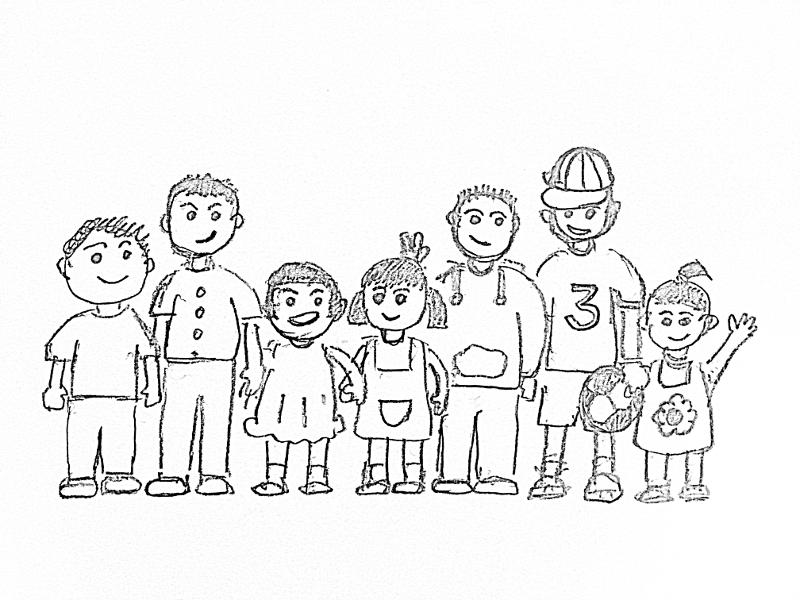
\includegraphics[scale=0.3]{img/kids}
 \captionsetup{labelformat = empty}
 \label{fig:kids-sort}
\end{figure}

Consider arrange kids in a line ordered by height.

\begin{enumerate}
\item The first kid raises hand, all shorter ones move to left, and the others move to right;
\item All kids on the left and right repeat.
\end{enumerate}

For example, the heights (in cm) are $[102, 100, 98, 95, 96, 99, 101, 97]$. \Cref{tab:kids-sort} gives the steps. (1) The kid of 102 cm raises hand as the pivot (underlined in the first row). He happens to be the tallest, hence all others move to the left as shown in the second row in the table. (2) The kid of 100 cm is the pivot. Those of height 98, 95, 96, and 99 cm move to the left, and the one of 101 cm moves to the right, as shown in the third row. (3) The kid of 98 cm is the left pivot, while 101 cm is the right pivot. Because there is only one kid on the right, it's sorted. Repeat this to sort all kids.

\begin{table}[htbp]
\centering
\begin{tabular}{ | c c c c c c c c |}
\hline
\underline{102} & 100 & 98 & 95 & 96 & 99 & 101 & 97 \\
\underline{100} & 98 & 95 & 96 & 99 & 101 & 97 & `102' \\
\underline{98} & 95 & 96 & 99 & 97 & `100' & 101 & `102' \\
\underline{95} & 96 & 97 & `98' & 99 & `100' & `101' & `102' \\
`95' & \underline{96} & 97 & `98' & `99' & `100' & `101' & `102' \\
`95' & `96' & 97 & `98' & `99' & `100' & `101' & `102' \\
`95' & `96' & `97' & `98' & `99' & `100' & `101' & `102' \\
\hline
\end{tabular}
\caption{Sort steps}
\label{tab:kids-sort}
\end{table}

Summarize the quick sort. Let the list be $L$:

\begin{itemize}
\item If $L$ is empty$[\ ]$, the result is $[\ ]$;
\item Otherwise, select an element as the pivot $p$, recursively sort elements $\leq p$ to the left; {\em and} sort other elements $> p$ to the right.
\end{itemize}

We say {\em and}, but not `then', indicate we can sort left and right in parallel. C. A. R. Hoare developed quick sort in 1960\cite{TAOCP}\cite{wiki-qs}. There are varies of ways to pick the pivot, for example, always choose the first element.

\be
\begin{array}{rcl}
sort\ [\ ] & = & [\ ] \\
sort\ (x \cons xs) & = & sort\ [y \gets xs, y \leq x] \doubleplus [x] \doubleplus sort\ [y \gets xs, x < y] \\
\end{array}
\ee

We use ZF expression (see \cref{sec:zf-expr,sec:list-filter}) to filter the list. Below is the example program:

\lstset{frame = single}
\begin{Haskell}
sort [] = []
sort (x:xs) = sort [y | y<-xs, y <= x] ++ [x] ++ sort [y | y<-xs, x < y]
\end{Haskell}

We assume to sort in ascending order. We can abstract the ($\leq$) as generic comparison to sort different things like numbers, strings, and etc. We needn't total ordering, but at least need {\em strict weak ordering}\cite{wiki-total-order}\cite{wiki-sweak-order}(see \cref{sec:strict-weak-order}).

\subsection{Partition}
\index{Quick sort!partition}
We traverse the elements in two passes: first filter all elements $\leq x$ ; next filter all $> x$. Let us combine them into one pass:

\be
\begin{array}{rcl}
\textit{part}\ p\ [\ ] & = & ([\ ], [\ ]) \\
\textit{part}\ p\ (x \cons xs) & = & \begin{cases}
 p(x): & (x \cons as, bs), \text{where}\ (as, bs) = \textit{part}\ p\ xs \\
 \text{otherwise}: & (as, x \cons bs) \\
\end{cases} \\
\end{array}
\label{eq:qsort-partition}
\ee

And change the quick sort to:

\be
\begin{array}{rcl}
sort\ [\ ] & = & [\ ] \\
sort\ (x \cons xs) & = & sort\ as \doubleplus [x] \doubleplus sort\ bs, \text{where}\ (as, bs) = \textit{part}\ (\leq x)\ xs \\
\end{array}
\ee

Alternatively, we can define partition with fold (in Curried form):

\be
\textit{part}\ p\ = foldr\ f\ ([\ ], [\ ])
\ee

Where:

\be
f\ (as, bs)\ x = \begin{cases}
p(x): & (x \cons as, bs) \\
\text{otherwise}: & (as, x \cons bs) \\
\end{cases}
\ee

It's essentially to accumulate to $(as, bs)$. If $p(x)$ holds, then add $x$ to $as$, otherwise to $bs$. Change the partition to tail recursive:

\be
\begin{array}{rcl}
\textit{part}\ p\ [\ ]\ as\ bs & = & (as, bs) \\
\textit{part}\ p\ (x \cons xs)\ as\ bs & = & \begin{cases}
  p(x): & \textit{part}\ p\ xs\ (x \cons as)\ bs \\
  \text{otherwise}: & \textit{part}\ p\ xs\ as\ (x \cons bs) \\
\end{cases}
\end{array}
\ee

To partition $(x \cons xs)$, call $(as, bs) = \textit{part}\ (\leq x)\ xs\ [\ ]\ [\ ]$. We eliminate the concatenation ($\doubleplus$) in `$sort\ as \doubleplus [x] \doubleplus sort\ bs$' with an accumulators $s$ as:

\be
\begin{array}{rcl}
sort'\ s\ [\ ] & = & s \\
sort'\ s\ (x \cons xs) & = & sort'\ (x : sort'\ s\ bs)\ as \\
\end{array}
\ee

Start it with an empty list: $sort = sort'\ [\ ]$. After partition, we need recursively sort $as, bs$. We can first sort $bs$, prepend $x$, then pass it as the new accumulator to sort $as$:

\begin{Haskell}
sort = sort' []

sort' s [] = s
sort' s (x:xs) = sort' (x : sort' s bs) as where
  (as, bs) = part xs [] []
  part [] as bs = (as, bs)
  part (y:ys) as bs | y <= x = part ys (y:as) bs
                    | otherwise = part ys as (y:bs)
\end{Haskell}

\subsection{In-place sort}

\Cref{fig:partition-1-way} gives a way to partition in-place\cite{Bentley}\cite{CLRS}. Scan from left to right. At any time, the array is consist of four parts (\cref{fig:partition-1-way} (a)):

\begin{figure}[htbp]
   \centering
   \subcaptionbox{Partition invariant}{
      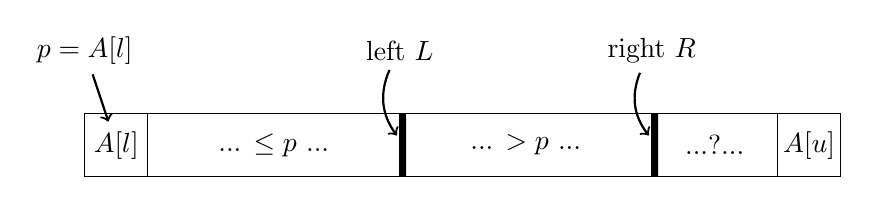
\begin{tikzpicture}[scale=0.8]
      \draw (0, 0) rectangle (1, 1) node (xl) [pos=.5] {$A[l]$}
            (1, 0) rectangle (5, 1) node (leq) [pos=.5] {... $\leq p$ ...}
            (5, 0) rectangle (9, 1) node (ge) [pos=.5] {... $> p$ ...}
            (9, 0) rectangle (11, 1) node (rest) [pos=.5] {...?...}
            (11, 0) rectangle (12, 1) node (xu) [pos=.5] {$A[u]$};
      \fill [black] (5, 0) rectangle (5.1, 1) node (leftbar) [pos=.5] {}
                    (9, 0) rectangle (9.1, 1) node (rightbar) [pos=.5] {};
      \draw (0, 2) node (pivot) {$p = A[l]$}
            (5, 2) node (left) {left $L$}
            (9, 2) node (right) {right $R$};
      \draw[thick, ->] (pivot) edge (xl)
                       (left) edge [bend right] (leftbar)
                       (right) edge [bend right] (rightbar);
      \end{tikzpicture}} \\
   \subcaptionbox{Initialize}{
      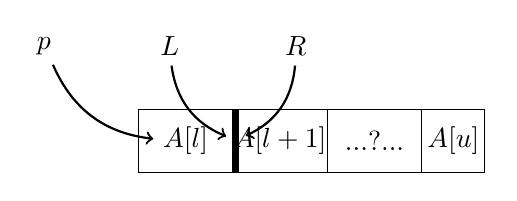
\begin{tikzpicture}[scale=0.8]
      \draw (-0.5, 0) rectangle (1, 1) node (xl) [pos=.5] {$A[l]$}
            (1, 0) rectangle (2.5, 1) node (xl1) [pos=.5] {$A[l+1]$}
            (2.5, 0) rectangle (4, 1) node (rest) [pos=.5] (ai) {...?...}
            (4, 0) rectangle (5, 1) node (xu) [pos=.5] {$A[u]$};
      \fill [black] (1, 0) rectangle (1.1, 1) node (leftbar) [pos=.5] {};
      \draw (-2, 2) node (pivot) {$p$}
            (0, 2) node (left) {$L$}
            (2, 2) node (right) {$R$};
      \draw[thick, ->] (pivot) edge [bend right] (xl)
                       (left) edge [bend right] (leftbar)
                       (right) edge [bend left] (leftbar);
      \end{tikzpicture}} \\
   \subcaptionbox{Terminate}{
      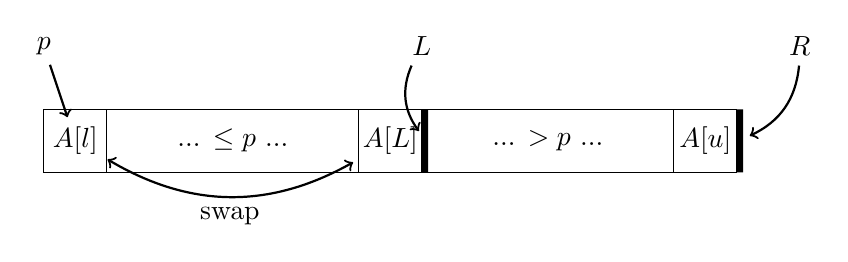
\begin{tikzpicture}[scale=0.8]
      \draw (0, 0) rectangle (1, 1) node (xl) [pos=.5] {$A[l]$}
            (1, 0) rectangle (5, 1) node (leq) [pos=.5] {... $\leq p$ ...}
            (5, 0) rectangle (6, 1) node (xleft) [pos=.5] {$A[L]$}
            (6, 0) rectangle (10, 1) node (ge) [pos=.5] {... $> p$ ...}
            (10, 0) rectangle (11, 1) node (xu) [pos=.5] {$A[u]$};
      \fill [black] (6, 0) rectangle (6.1, 1) node (leftbar) [pos=.5] {}
                    (11, 0) rectangle (11.1, 1) node (rightbar) [pos=.5] {};
      \draw (0, 2) node (pivot) {$p$}
            (6, 2) node (left) {$L$}
            (12, 2) node (right) {$R$};
      \draw[thick, ->] (pivot) edge (xl)
                       (left) edge [bend right] (leftbar)
                       (right) edge [bend left] (rightbar);
      \draw[thick, <->] (xl) edge [bend right] node [below] {swap} (xleft);
      \end{tikzpicture}} \\
   \caption{In-place partition, pivot $p = A[l]$}
   \label{fig:partition-1-way}
\end{figure}

\begin{enumerate}
\item The pivot is the left element: $p = A[l]$. It moves to the final position after partition;
\item A section of elements $\leq p$, extends right to $L$;
\item A section of elements $> p$, extends right to $R$. The elements between $L$ and $R$ are $> p$;
\item Elements after $R$ haven't been partitioned (maybe $>$ or $=$ or $< p$).
\end{enumerate}

When partition starts, $L$ points to $p$, $R$ points to the next (\cref{fig:partition-1-way} (b)). We advance $R$ to the right boundary. Every time, compare $A[R]$ and $p$. If $A[R] > p$, it should be between $L$ and $R$, we move $R$ forward; otherwise if $A[R] \leq p$, it should be on the left of $L$. We advance $L$ a step, then swap $A[L] \leftrightarrow A[R]$. The partition ends when $R$ passes the last element. All elements $> p$ are moved to the right of $L$, while others are on the left. We need move $p$ to the position between the two parts. To do that, swap $p \leftrightarrow A[L]$, as shown in \cref{fig:partition-1-way} (c). $L$ finally points to $p$, partitioned the array in two parts. We return $L + 1$ as the result, that points to the first element $> p$. Let the array be $A$, the lower, upper boundaries be $l, u$. The in-place partition is defined below:

\begin{algorithmic}[1]
\Function{Partition}{$A, l, u$}
  \State $p \gets A[l]$  \Comment{pivot}
  \State $L \gets l$ \Comment{left}
  \For{$R$ in $[l+1, u]$} \Comment{iterate on right}
    \If{$p \geq A[R]$}
      \State $L \gets L + 1$
      \State \textproc{Exchange} $A[L] \leftrightarrow A[R]$
    \EndIf
  \EndFor
  \State \textproc{Exchange} $A[L] \leftrightarrow p$
  \State \Return $L + 1$ \Comment{partition position}
\EndFunction
\end{algorithmic}

\Cref{tab:partition-steps} lists the steps to partition $[3, 2, 5, 4, 0, 1, 6, 7]$.

\begin{table}[htbp]
\centering
\begin{tabular}{|llllllll|l|}
\hline
\underline{3}(l)  & 2(r) & 5 & 4 & 0 & 1 & 6 & 7 & start, $p = 3$, $l = 1$, $r = 2$ \\
\underline{3} & 2(l)(r) & 5 & 4 & 0 & 1 & 6 & 7 & $2 < 3$, advance $l$ ($r=l$) \\
\underline{3} & 2(l) & 5(r) & 4 & 0 & 1 & 6 & 7 & $5 > 3$, move on \\
\underline{3} & 2(l) & 5 & 4(r) & 0 & 1 & 6 & 7 & $4 > 3$, move on \\
\underline{3} & 2(l) & 5 & 4 & 0(r) & 1 & 6 & 7 & $0 < 3$ \\
\underline{3} & 2 & 0(l) & 4 & 5(r) & 1 & 6 & 7 & advance $l$, swap with $r$ \\
\underline{3} & 2 & 0(l) & 4 & 5 & 1(r) & 6 & 7 & $1 < 3$ \\
\underline{3} & 2 & 0 & 1(l) & 5 & 4(r) & 6 & 7 & advance $l$, swap with $r$ \\
\underline{3} & 2 & 0 & 1(l) & 5 & 4 & 6(r) & 7 & $6 > 3$, move on \\
\underline{3} & 2 & 0 & 1(l) & 5 & 4 & 6 & 7(r) & $7 > 3$, move on \\
1 & 2 & 0 & 3 & 5(l+1) & 4 & 6 & 7 & terminate, swap $p$ and $l$ \\
\hline
\end{tabular}
\caption{Partition array} \label{tab:partition-steps}
\end{table}

We implement quick sort with \textproc{Partition} as bellow:

\begin{algorithmic}[1]
\Procedure{Quick-Sort}{$A, l, u$}
  \If{$l < u$}
    \State $m \gets$ \Call{Partition}{$A, l, u$}
    \State \Call{Quick-Sort}{$A, l, m - 1$}
    \State \Call{Quick-Sort}{$A, m, u$}
  \EndIf
\EndProcedure
\end{algorithmic}

We pass the array and its boundaries as \textproc{Quick-Sort}($A, 1, |A|$) to sort. It returns immediately if the array is empty or a singleton.

\begin{Exercise}\label{ex:basic-qsort}
\Question{Optimize the basic quick sort definition for the singleton list case.}
\end{Exercise}

\begin{Answer}[ref = {ex:basic-qsort}]
\Question{Optimize the basic quick sort definition for the singleton list case.

Add a case:
\begin{Haskell}
sort [x] = [x]
\end{Haskell}
}
\end{Answer}

\subsection{Performance}
\index{Quick sort!Performance} \label{sec:quick-sort-big-o}

Quick sort performs well in most cases. Consider the best/worst cases. For the best case, it always halves the elements into two equal sized parts. As shown in figure \cref{fig:qsort-best}, there are total $O(\lg n)$ levels of recursions. At level one, it processes $n$ elements with one partition; at level two, partitions twice, each processes $n/2$ elements, taking total $2 O(n/2) = O(n)$ time; at level three, partitions four times, each processes $n/4$ elements, taking total $O(n)$ time too, ..., at the last level, there are $n$ singleton segments, taking total $O(n)$ time. Sum all levels, the time is bound to $O(n \lg n)$.

\begin{figure}[htbp]
 \centering
 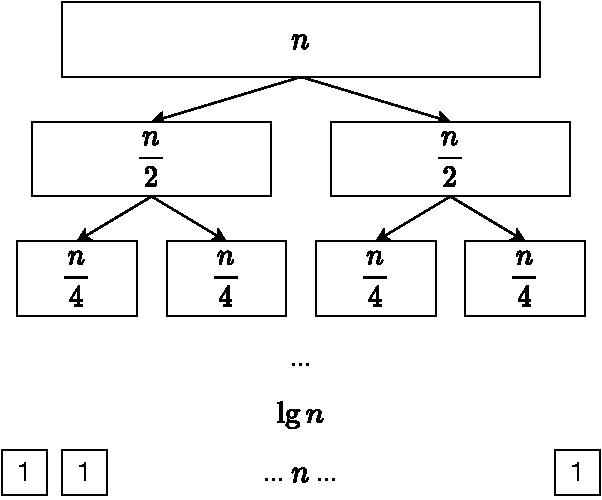
\includegraphics[scale=0.55]{img/qsort-best}
 \caption{The best case, halve every time.}
 \label{fig:qsort-best}
\end{figure}

For the worst case, the partition is totally unbalanced, one part is of $O(1)$ length, the other is $O(n)$. The level of recursions decays to $O(n)$. Model the partition as a tree. It's balanced binary tree in the best case, while it becomes a linked-list of $O(n)$ length in the worst case. Every branch node has an empty sub-tree. At each level, we process all elements, hence the total time is bound to $O(n^2)$. This is same as insertion sort, and selection sort. There are several challenging cases, for example, the sequence has many duplicated elements, or is largely ordered, and etc. There isn't a method can avoid the worst case completely.

\subsubsection{Average case\texorpdfstring{$\bigstar$}{★}}
\index{Quick Sort!Average case}

Quick sort performs well in average. For example, even if every partition gives two parts of 1:9, the performance still achieves $O(n \lg n)$\cite{CLRS}. We give two methods to evaluate the performance. The first one is based on the fact, that the performance is proportion to the number of comparisons. In selection sort, every two elements are compared, while in quick sort, we save many comparisons. When partition sequence $[a_1, a_2, a_3, ..., a_n]$ with $a_1$ as the pivot, we obtain two sub sequences $A = [x_1, x_2, ..., x_k]$ and $B = [y_1, y_2, ..., y_{n-k-1}]$. After that, none element $x_i$ in $A$ will be compared with any $y_j$ in $B$. Let the sorted result be $[a_1, a_2, ..., a_n]$, if $a_i < a_j$, we do not compare them if and only if there is some element $a_k$, where $a_i < a_k < a_j$, is picked as the pivot before either $a_i$ or $a_j$ being the pivot. In other word, the only chance that we compare $a_i$ and $a_j$ is either $a_i$ or $a_j$ is chosen as the pivot before any other elements in $a_{i+1} < a_{i+2} < ... < a_{j-1}$ being the pivot. Let $P(i, j)$ be the probability that we compare $a_i$ and $a_j$. We have:

\be
P(i, j) = \frac{2}{j - i + 1}
\ee

The total number of comparisons is:

\be
C(n) = \sum_{i=1}^{n-1}\sum_{j=i+1}^{n} P(i, j)
\ee

If we compare $a_i$ and $a_j$, we won't compare $a_j$ and $a_i$ again, and we never compare $a_i$ with itself. The upper bound of $i$ is $n-1$, and the lower bound of $j$ is $i+1$. Substitute the probability:

\be
\begin{array}{rl}
C(n) & = \displaystyle \sum_{i=1}^{n-1}\sum_{j = i+1}^{n} \frac{2}{j - i + 1} \\
     & = \displaystyle \sum_{i=1}^{n-1}\sum_{k=1}^{n-i} \frac{2}{k+1} \\
\end{array}
\ee

Use the result of harmonic series\cite{wiki-harmonic}.

\[
H_n = 1 + \frac{1}{2} + \frac{1}{3} + .... = \ln n + \gamma + \epsilon_n
\]

\be
C(n) = \sum_{i=1}^{n-1} O(\lg n) = O(n \lg n)
\ee

The other method uses the recursion. Let the length of the sequence be $n$, we partition it into two parts of length $i$ and $n-i-1$. The partition takes $cn$ time because it compares every element with the pivot. The total time is:

\be
T(n) = T(i) + T(n-i-1) + c n
\ee

Where $T(n)$ is the time to sort $n$ elements. $i$ equally distributes across $0, 1, ..., n-1$. Taking math expectation:

\be
\renewcommand*{\arraystretch}{1.5}
\begin{array}{rl}
T(n) & = E(T(i)) + E(T(n-i-1)) + c n \\
     & = \displaystyle \frac{1}{n} \sum_{i=0}^{n-1}T(i) + \frac{1}{n} \sum_{i=0}^{n-1}T(n-i-1) + cn \\
     & = \displaystyle \frac{1}{n} \sum_{i=0}^{n-1}T(i) + \frac{1}{n} \sum_{j=0}^{n-1}T(j) + cn \\
     & = \displaystyle \frac{2}{n} \sum_{i=0}^{n-1}T(i) + cn
\end{array}
\ee

Multiply $n$ to both sides:

\be
n T(n) = 2 \sum_{i=0}^{n-1} T(i) + c n^2
\label{eq:ntn}
\ee

Substitute $n$ to $n-1$:

\be
(n-1) T(n-1) = 2 \sum_{i=0}^{n-2} T(i) + c (n-1)^2
\label{eq:n1tn1}
\ee

Take (\cref{eq:ntn}) - (\cref{eq:n1tn1}), cancel all $T(i)$ for $0 \leq i < n-1$.

\be
n T(n) = (n + 1) T(n-1) + 2cn - c
\ee

Drop the constant $c$, we obtain:

\be
\frac{T(n)}{n+1} = \frac{T(n-1)}{n} + \frac{2c}{n+1}
\ee

Assign $n$ to $n-1$, $n-2$, ..., to give $n-1$ equations.

\[
\frac{T(n-1)}{n} = \frac{T(n-2)}{n-1} + \frac{2c}{n}
\]

\[
\frac{T(n-2)}{n-1} = \frac{T(n-3)}{n-2} + \frac{2c}{n-1}
\]

\[
...
\]

\[
\frac{T(2)}{3} = \frac{T(1)}{2} + \frac{2c}{3}
\]

Sum up and cancel the same components on both sides, we get a function of $n$.

\be
\frac{T(n)}{n+1} = \frac{T(1)}{2} + 2c \sum_{k=3}^{n+1} \frac{1}{k}
\ee

Use the result of the harmonic series:

\be
O(\frac{T(n)}{n+1}) = O(\frac{T(1)}{2} + 2c \ln n + \gamma + \epsilon_n) = O(\lg n)
\ee

Therefore:

\be
O(T(n)) = O(n \lg n)
\ee

\subsection{Improvement}
\index{Quick sort!Improvement} \index{Quick sort!Ternary partition}

The \textproc{Partition} procedure doesn't perform well when there are many duplicated elements. Consider the extreme case that all $n$ elements are equal $[x, x, ..., x]$:

\begin{enumerate}
\item From the quick sort definition: pick any element as the pivot, hence $p = x$, partition into two sub-sequences. One is $[x, x, ..., x]$ of length $n - 1$, the other is empty. Next recursively sort the $n-1$ elements, the total time decays to $O(n^2)$.
\item Modify the partition with $< x$ and $> x$. The result are two empty sub-sequences, and $n$ elements equal to $x$. The recursion on empty sequence terminates immediately. The result is $[\ ] \doubleplus [x, x, ..., x] \doubleplus [\ ]$. The performance is $O(n)$.
\end{enumerate}

We improve from {\em binary} partition to {\em ternary} partition to handle the duplicated elements:

\be
\begin{array}{rcl}
sort\ [\ ] & = & [\ ] \\
sort\ (x \cons xs) & = & sort\ S \doubleplus sort\ E \doubleplus sort\ G
\end{array}
\ee

Where:

\[
\begin{cases}
S = [ y \gets xs, y < x ] \\
E = [ y \gets xs, y = x ] \\
G = [ y \gets xs, y > x ] \\
\end{cases}
\]

we use an accumulator to improve the list concatenation: $qsort = sort\ [\ ]$, where:

\be
\begin{array}{rcl}
sort\ A\ [\ ] & = & A \\
sort\ A\ (x \cons xs) & = & sort\ (E \doubleplus sort\ A\ G)\ S \\
\end{array}
\ee

The sub-list $E$ contains elements of the same value, hence sorted. We first sort $G$ with the accumulator $A$, then prepend $E$ as the new accumulator, and use it to sort $S$. We also improve the partition with accumulator:

\be
\begin{array}{rcl}
part\ S\ E\ G\ x\ [\ ] & = & (S, E, G) \\
part\ S\ E\ G\ x\ (y \cons ys) & = & \begin{cases}
  y < x: & (y \cons S, E, G) \\
  y = x: & (S, y \cons E, G) \\
  y > x: & (S, E, y \cons G) \\
  \end{cases} \\
\end{array}
\ee

Richard Bird gives another improvement\cite{fp-pearls}: collect the recursive sort results with a list and concatenate it finally:

\begin{Haskell}
sort :: (Ord a) => [a] -> [a]
sort = concat . (pass [])

pass xss [] = xss
pass xss (x:xs) = step xs [] [x] [] xss where
    step [] as bs cs xss = pass (bs : pass xss cs) as
    step (x':xs') as bs cs xss | x' <  x = step xs' (x':as) bs cs xss
                               | x' == x = step xs' as (x':bs) cs xss
                               | x' >  x = step xs' as bs (x':cs) xss
\end{Haskell}

\index{Quick Sort!2-way partition}
Robert Sedgewick develops the two-way partition method\cite{qsort-impl}\cite{Bentley}. Use two pointers $i, j$ to the left and right boundaries. Pick the first element as the pivot $p$. Advance $i$ to right till meet an element $\geq p$; while (in parallel) move $j$ to left till meet an element $\leq p$. At this time, all elements on the left to $i$ are less than the pivot ($< p$), while those on the right to $j$ are greater than the pivot ($> p$). $i$ points to an element that is $\geq p$, and $j$ points to an element that is $\leq p$, as shown in \cref{fig:partition-2-way} (a). To move all elements $\leq p$ to the left, and the remaining to the right, we exchange $x[i] \leftrightarrow x[j]$, then continue scan. Repeat this till $i$ meets $j$. At any time, we keep the invariant: all elements one the left to $i$ (include $i$) are $\leq p$; while all on the right to $j$ (include $j$) are $\geq p$. The elements between $i$ and $j$ are yet to scan, as shown in \cref{fig:partition-2-way} (b).

\begin{figure}[htbp]
   \centering
   \subcaptionbox{When $i$ and $j$ stop}{
      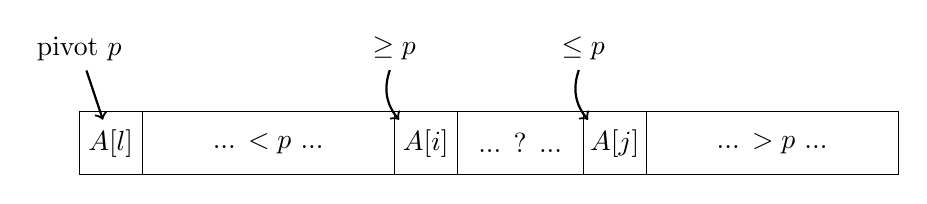
\begin{tikzpicture}[scale=0.8]
      \draw (0, 0) rectangle (1, 1) node (xl) [pos=.5] {$A[l]$}
            (1, 0) rectangle (5, 1) node (leq) [pos=.5] {... $< p$ ...}
            (5, 0) rectangle (6, 1) node (xi) [pos=.5] {$A[i]$}
            (6, 0) rectangle (8, 1) node (rest) [pos=.5] {... ? ...}
            (8, 0) rectangle (9, 1) node (xj) [pos=.5] {$A[j]$}
            (9, 0) rectangle (13, 1) node (ge) [pos=.5] {... $> p$ ...};
      \draw (0, 2) node (pivot) {pivot $p$}
            (5, 2) node (left) {$\geq p$}
            (8, 2) node (right) {$\leq p$};
      \draw[thick, ->] (pivot) edge (xl)
                       (left) edge [bend right] (xi)
                       (right) edge [bend right] (xj);
      \end{tikzpicture}} \\
   \subcaptionbox{Partition invariant}{
      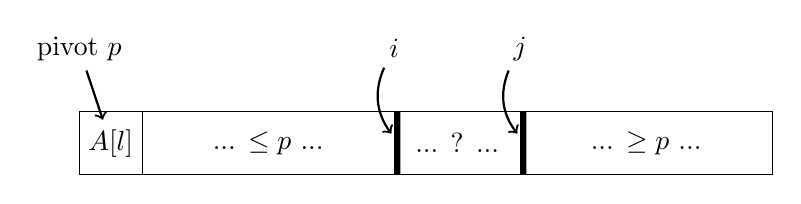
\begin{tikzpicture}[scale=0.8]
      \draw (0, 0) rectangle (1, 1) node (xl) [pos=.5] {$A[l]$}
            (1, 0) rectangle (5, 1) node (leq) [pos=.5] {... $\leq p$ ...}
            (5, 0) rectangle (7, 1) node (rest) [pos=.5] {... ? ...}
            (7, 0) rectangle (11, 1) node (ge) [pos=.5] {... $\geq p$ ...};
      \fill [black] (5, 0) rectangle (5.1, 1) node (ibar) [pos=.5] {}
                    (7, 0) rectangle (7.1, 1) node (jbar) [pos=.5] {};
      \draw (0, 2) node (pivot) {pivot $p$}
            (5, 2) node (i) {$i$}
            (7, 2) node (j) {$j$};
      \draw[thick, ->] (pivot) edge (xl)
                       (i) edge [bend right] (ibar)
                       (j) edge [bend right] (jbar);
      \end{tikzpicture}} \\
   \caption{2-way scan}
   \label{fig:partition-2-way}
\end{figure}

When $i$ meets $j$, we need an additional exchange: swap the pivot $p$ to position $j$. Then recursive sort the sub-arrays $A[l ... j)$ and $A[i ... u)$.

\begin{algorithmic}[1]
\Procedure{Sort}{$A, l, u$} \Comment{Sort range $[l, u)$}
  \If{$u - l > 1$} \Comment{At least 2 elements}
    \State $i \gets l$, $j \gets u$
    \State $pivot \gets A[l]$
    \Loop
      \Repeat
        \State $i \gets i + 1$
      \Until{$A[i] \geq pivot$} \Comment{Ignore $i \geq u$}
      \Repeat
        \State $j \gets j - 1$
      \Until{$A[j] \leq pivot$} \Comment{Ignore $j < l$}
      \If{$j < i$}
        \State break
      \EndIf
      \State \textproc{Exchange} $A[i] \leftrightarrow A[j]$
    \EndLoop
    \State \textproc{Exchange} $A[l] \leftrightarrow A[j]$ \Comment{Move the pivot}
    \State \Call{Sort}{$A, l, j$}
    \State \Call{Sort}{$A, i, u$}
  \EndIf
\EndProcedure
\end{algorithmic}

\index{Quick Sort!3-way partition}
For the extreme case that all elements are equal, the array is partitioned into two same parts with $\dfrac{n}{2}$ swaps. Because of the balanced partition, the performance is $O(n \lg n)$. It takes less swaps than the one pass scan method, since it skips the elements on the right side of the pivot. We can combine the 2-way scan and the ternary partition. Only recursively sort the elements different with the pivot. Jon Bentley and Douglas McIlroy develop a method as shown in \cref{fig:partition-3-way} (a), that store the elements equal to the pivot on both sides\cite{3-way-part}\cite{opt-qs}.

\begin{figure}[htbp]
   \centering
   \subcaptionbox{Ternary partition invariant.}{
      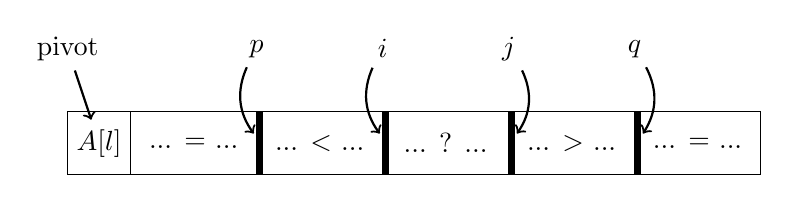
\begin{tikzpicture}[scale=0.8]
      \draw (0, 0) rectangle (1, 1) node (xl) [pos=.5] {$A[l]$}
            (1, 0) rectangle (3, 1) node [pos=.5] {... $=$ ...}
            (3, 0) rectangle (5, 1) node [pos=.5] {... $<$ ...}
            (5, 0) rectangle (7, 1) node [pos=.5] {... ? ...}
            (7, 0) rectangle (9, 1) node [pos=.5] {... $>$ ...}
            (9, 0) rectangle (11, 1) node [pos=.5] {... $=$ ...};
      \fill [black] (3, 0) rectangle (3.1, 1) node (pbar) [pos=.5] {}
                    (5, 0) rectangle (5.1, 1) node (ibar) [pos=.5] {}
                    (7, 0) rectangle (7.1, 1) node (jbar) [pos=.5] {}
                    (9, 0) rectangle (9.1, 1) node (qbar) [pos=.5] {};
      \draw (0, 2) node (pivot) {pivot}
            (3, 2) node (p) {$p$}
            (5, 2) node (i) {$i$}
            (7, 2) node (j) {$j$}
            (9, 2) node (q) {$q$};
      \draw[thick, ->] (pivot) edge (xl)
                       (p) edge [bend right] (pbar)
                       (i) edge [bend right] (ibar)
                       (j) edge [bend left] (jbar)
                       (q) edge [bend left] (qbar);
      \end{tikzpicture}} \\
   \subcaptionbox{Swap the elements $= p$ to the middle.}{\hspace{0.1\textwidth}
      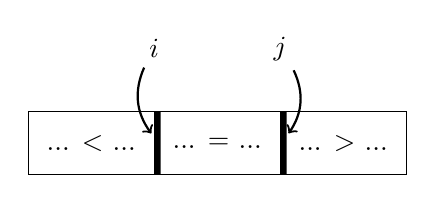
\begin{tikzpicture}[scale=0.8]
      \draw (0, 0) rectangle (2, 1) node [pos=.5] {... $<$ ...}
            (2, 0) rectangle (4, 1) node [pos=.5] {... $=$ ...}
            (4, 0) rectangle (6, 1) node [pos=.5] {... $>$ ...};
      \fill [black] (2, 0) rectangle (2.1, 1) node (ibar) [pos=.5] {}
                    (4, 0) rectangle (4.1, 1) node (jbar) [pos=.5] {};
      \draw (2, 2) node (i) {$i$}
            (4, 2) node (j) {$j$};
      \draw[thick, ->] (i) edge [bend right] (ibar)
                       (j) edge [bend left] (jbar);
      \end{tikzpicture}
      \hspace{0.1\textwidth}}
   \caption{Ternary partition}
   \label{fig:partition-3-way}
\end{figure}

We scan from two sides, pause when $i$ reaches an element $\geq$ the pivot, and $j$ reaches one $\leq$ the pivot. If $i$ doesn't meet or pass $j$, we exchange $A[i] \leftrightarrow A[j]$, then check if $A[i]$ or $A[j]$ equals to the pivot. If yes, we exchange $A[i] \leftrightarrow A[p]$ or $A[j] \leftrightarrow A[q]$ respectively. Finally, we swap all the elements equal to the pivot to the middle. This step does nothing if all elements are distinct. The partition result is shown as \cref{fig:partition-3-way} (b). We next only recursively sort the elements not equal to the pivot.

\begin{algorithmic}[1]
\Procedure{Sort}{$A, l, u$}
  \If{$u - l > 1$}
    \State $i \gets l$, $j \gets u$
    \State $p \gets l$, $q \gets u$ \Comment{point to the boundaries of duplicated elements}
    \State $pivot \gets A[l]$
    \Loop
      \Repeat
        \State $i \gets i + 1$
      \Until{$A[i] \geq pivot$} \Comment{Ignore $i \geq u$ case}
      \Repeat
        \State $j \gets j - 1$
      \Until{$A[j] \leq pivot$} \Comment{Ignore $j < l$ case}
      \If{$j \leq i$}
        \State break
      \EndIf
      \State \textproc{Exchange} $A[i] \leftrightarrow A[j]$
      \If{$A[i] = pivot$} \Comment{duplicated element}
        \State $p \gets p + 1$
        \State \textproc{Exchange} $A[p] \leftrightarrow A[i]$
      \EndIf
      \If{$A[j] = pivot$}
        \State $q \gets q - 1$
        \State \textproc{Exchange} $A[q] \leftrightarrow A[j]$
      \EndIf
    \EndLoop
    \If{$i = j$ and $A[i] = pivot$}
      \State $j \gets j - 1$, $i \gets i + 1$
    \EndIf
    \For{$k$ from $l$ to $p$} \Comment{Swap the duplicated elements to the middle}
      \State \textproc{Exchange} $A[k] \leftrightarrow A[j]$
      \State $j \gets j - 1$
    \EndFor
    \For{$k$ from $u-1$ down-to $q$}
      \State \textproc{Exchange} $A[k] \leftrightarrow A[i]$
      \State $i \gets i + 1$
    \EndFor
    \State \Call{Sort}{$A, l, j + 1$}
    \State \Call{Sort}{$A, i, u$}
  \EndIf
\EndProcedure
\end{algorithmic}

It becomes complex when combine the 2-way scan and the ternary partition. Alternatively, we change the one pass scan to the ternary partition directly. Pick the first element as the pivot, as shown in \cref{fig:partition-3-way-lomuto}. At any time, the left part contains elements $< p$; the next part contains those $= p$; and the right part contains those $> p$. The boundaries are $i, k, j$. Elements between $[k, j)$ are yet to be partitioned. We scan from left to right. When start, the part $< p$ is empty; the part $= p$ has an element; $i$ points to the lower boundary, $k$ points to the next. The part $> p$ is empty too, $j$ points to the upper boundary.

\begin{figure}[htbp]
   \centering
      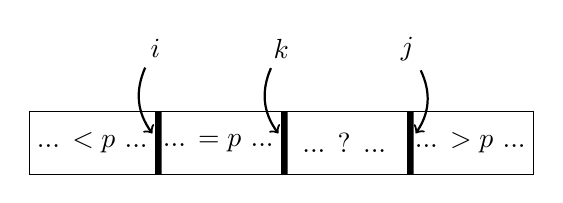
\begin{tikzpicture}[scale=0.8]
      \draw (0, 0) rectangle (2, 1) node [pos=.5] {... $< p$ ...}
            (2, 0) rectangle (4, 1) node [pos=.5] {... $= p$ ...}
            (4, 0) rectangle (6, 1) node [pos=.5] {... ? ...}
            (6, 0) rectangle (8, 1) node [pos=.5] {... $> p$ ...};
      \fill [black] (2, 0) rectangle (2.1, 1) node (ibar) [pos=.5] {}
                    (4, 0) rectangle (4.1, 1) node (kbar) [pos=.5] {}
                    (6, 0) rectangle (6.1, 1) node (jbar) [pos=.5] {};
      \draw (2, 2) node (i) {$i$}
            (4, 2) node (k) {$k$}
            (6, 2) node (j) {$j$};
      \draw[thick, ->] (i) edge [bend right] (ibar)
                       (k) edge [bend right] (kbar)
                       (j) edge [bend left] (jbar);
      \end{tikzpicture}
   \caption{1 way scan ternary partition}
   \label{fig:partition-3-way-lomuto}
\end{figure}

Iterate on $k$, if $A[k] = p$, then move $k$ to the next; if $A[k] > p$, then exchange $A[k] \leftrightarrow A[j-1]$, the range of elements that $> p$ increases by one. Its boundary $j$ moves to left a step. Because we don't know if the element moved to $k$ is still $> p$, we need compare again and repeat. Otherwise if $A[k] < p$, we exchange $A[k] \leftrightarrow A[i]$, where $A[i]$ is the first element that $= p$. The partition terminates when $k$ meets $j$.

\begin{algorithmic}[1]
\Procedure{Sort}{$A, l, u$}
  \If{$u - l > 1$}
    \State $i \gets l$, $j \gets u$, $k \gets l + 1$
    \State $pivot \gets A[i]$
    \While{$k < j$}
      \While{$pivot < A[k]$}
        \State $j \gets j - 1$
        \State \textproc{Exchange} $A[k] \leftrightarrow A[j]$
      \EndWhile
      \If{$A[k] < pivot$}
        \State \textproc{Exchange} $A[k] \leftrightarrow A[i]$
        \State $i \gets i + 1$
      \EndIf
      \State $k \gets k + 1$
    \EndWhile
    \State \Call{Sort}{$A, l, i$}
    \State \Call{Sort}{$A, j, u$}
  \EndIf
\EndProcedure
\end{algorithmic}

This implementation is less complex but need more swaps than the version of ternary partition through 2-way scan.

\subsubsection{Challenging cases}

Although ternary partition handles duplicated elements well, there are other challenging cases. For example, when most elements are ordered (ascending or descending), the partition is unbalanced. \Cref{fig:worst-cases-1} gives two cases: $[x_1 < x_2 < ... < x_n]$ and $[y_1 > y_2 > ... > y_n]$. It's easy to give more, for example: $[x_m, x_{m-1}, ..., x_2, x_1, x_{m+1}, x_{m+2}, ... x_n]$, where $[ x_1 < x_2 < ... < x_n]$, and $[x_n, x_1, x_{n-1}, x_2, ... ]$ as shown in \cref{fig:worst-cases-2}.

\begin{figure}[htbp]
   \centering
   \subcaptionbox{Partition tree of $[x_1 < x_2 < ... < x_n]$, the sub-trees of $\leq p$ are empty.}{\hspace{.3\textwidth} 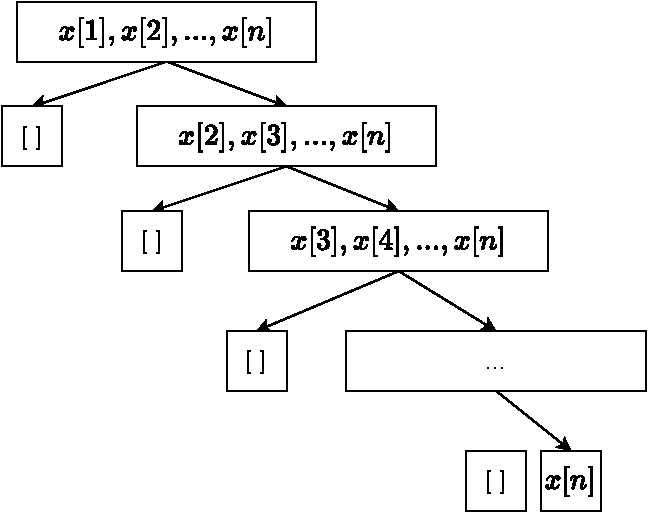
\includegraphics[scale=0.5]{img/unbalanced} \hspace{.3\textwidth}} \\
   \subcaptionbox{Partition tree of $[y_1 > y_2 > ... > y_n]$, the sub-trees of $\geq p$ are empty.}{\hspace{.3\textwidth} 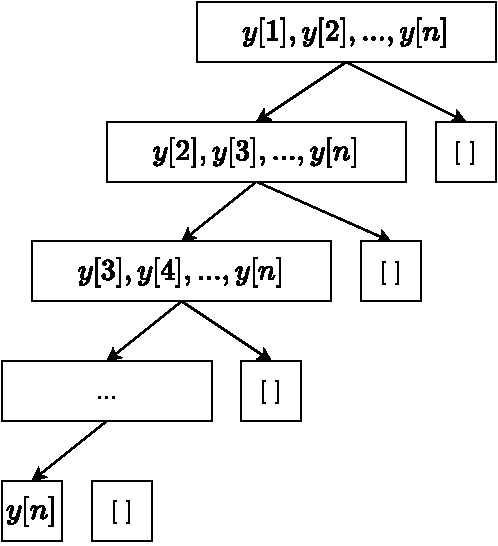
\includegraphics[scale=0.5]{img/unbalanced-2} \hspace{.3\textwidth}} \\
   \caption{The challenging cases - 1.}
   \label{fig:worst-cases-1}
\end{figure}

\begin{figure}[htbp]
   \centering
   \subcaptionbox{Unbalanced partitions except for the first time.}{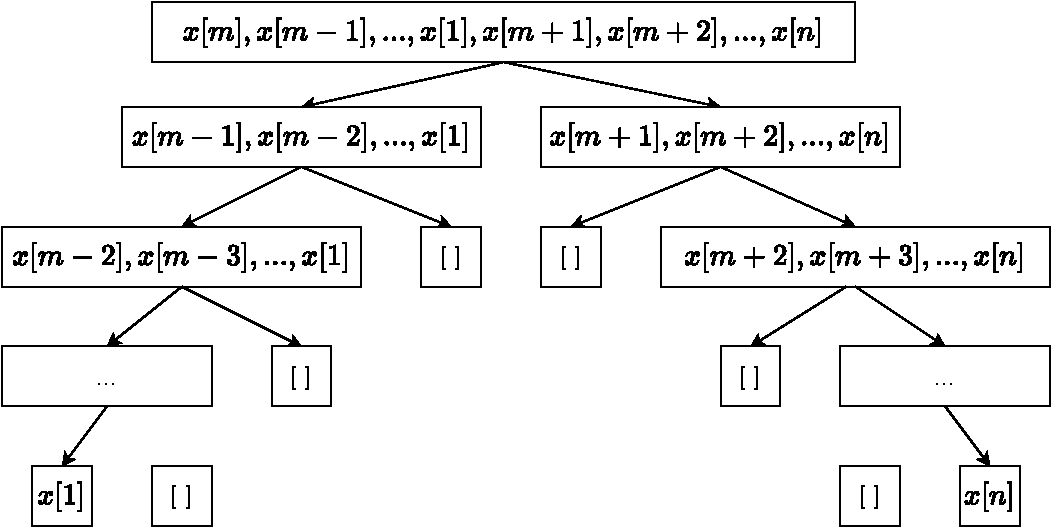
\includegraphics[scale=0.5]{img/unbalanced-3}} \\
   \subcaptionbox{A zig-zag partition tree.}{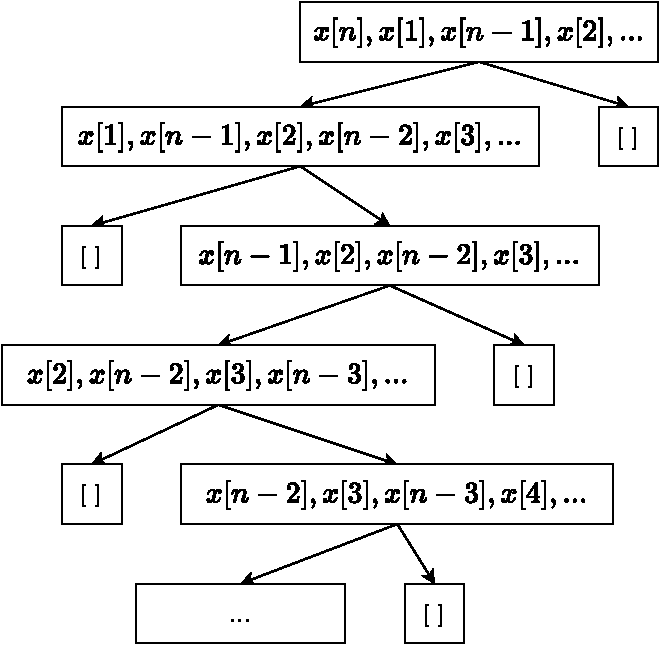
\includegraphics[scale=0.5]{img/unbalanced-zigzag}} \\
   \caption{The challenging cases - 2.}
   \label{fig:worst-cases-2}
\end{figure}

In these challenging cases, the partition is unbalanced when choose the first element as the pivot. Robert Sedgwick improves the pivot selection\cite{qsort-impl}: Instead pick a fixed position, sample several elements to avoid bad pivot. We sample the first, the middle, and the last, pick the median as the pivot. We can either compare every two (total 3 times)\cite{3-way-part}, or swap the least one to head, swap the greatest one to end, and move the median to the middle.

\begin{algorithmic}[1]
\Procedure{Sort}{$A, l, u$}
  \If{$u - l > 1$}
    \State $m \gets \lfloor \dfrac{l + u}{2} \rfloor$ \Comment{or $l + \dfrac{u - l}{2}$ to void overflow}
    \If{$A[m] < A[l]$} \Comment{Ensure $A[l] \leq A[m]$}
      \State \textproc{Exchange} $A[l] \leftrightarrow A[m]$
    \EndIf
    \If{$A[u-1] < A[l]$} \Comment{Ensure $A[l] \leq A[u-1]$}
      \State \textproc{Exchange} $A[l] \leftrightarrow A[u-1]$
    \EndIf
    \If{$A[u-1] < A[m]$} \Comment{Ensure $A[m] \leq A[u-1]$}
      \State \textproc{Exchange} $A[m] \leftrightarrow A[u-1]$
    \EndIf
    \State \textproc{Exchange} $A[l] \leftrightarrow A[m]$
    \State $(i, j) \gets $ \Call{Partition}{$A, l, u$}
    \State \Call{Sort}{$A, l, i$}
    \State \Call{Sort}{$A, j, u$}
  \EndIf
\EndProcedure
\end{algorithmic}

This implementation handles the above four challenging cases well, known as the `median of three'. Alternatively, we can randomly pick the pivot:

\begin{algorithmic}[1]
\Procedure{Sort}{$A, l, u$}
  \If{$u - l > 1$}
    \State \textproc{Exchange} $A[l] \leftrightarrow A[$ \Call{Random}{$l, u$} $]$
    \State $(i, j) \gets $ \Call{Partition}{$A, l, u$}
    \State \Call{Sort}{$A, l, i$}
    \State \Call{Sort}{$A, j, u$}
  \EndIf
\EndProcedure
\end{algorithmic}

Where \textproc{Random}($l, u$) returns integer $l \leq i < u$ randomly. We swap $A[i]$ with the first element as the pivot. This method is called {\em random quick sort} \cite{CLRS}. Theoretically, neither `median of three' nor random quick sort can avoid the worst case completely. If the sequence is random, it's same to choose any one as the pivot. Nonetheless, these improvements are widely used in engineering practice.

There are other improvements besides partition. Sedgewick find quick sort has overhead when the list is short, while insert sort performs better\cite{Bentley}\cite{3-way-part}. Sedgewick, Bentley and McIlroy evaluate varies thresholds, as `cut-off'. When the elements are less than the `cut-off', then switch to insert sort.

\begin{algorithmic}[1]
\Procedure{Sort}{$A, l, u$}
  \If{$u - l > $ \textproc{Cut-Off}}
    \State \Call{Quick-Sort}{$A, l, u$}
  \Else
    \State \Call{Insertion-Sort}{$A, l, u$}
  \EndIf
\EndProcedure
\end{algorithmic}

\subsection{quick sort and tree sort}

The `true quick sort' is the combination of multiple engineering improvements, e.g., falls back to insert sort for small sequence, in-place swaps, choose the pivot as the `median of three', 2-way scan, and ternary partition. Some people think the basic recursive definition is essentially tree sort. Richard Bird derives quick sort from binary tree sort by deforestation\cite{algo-fp}. Define \textit{unfold} that converts a list to binary search tree:

\be
\begin{array}{rcl}
\textit{unfold}\ [\ ] & = & \nil \\
\textit{unfold}\ (x \cons xs) & = & (\textit{unfold}\ [a \gets xs, a \leq x], x, \textit{unfold}\ [a \gets xs, a > x]) \\
\end{array}
\ee

Compare with the binary tree insert (see chapter 2), \textit{unfold} creates the tree differently. If the list is empty, the tree is empty; otherwise, use the first element $x$ as the key, then recursively build the left, and right sub-trees. Where the left sub-tree has the elements $\leq x$; and the right has the elements $> x$. Define in-order traverse to convert a binary search tree to ordered list:

\be
\begin{array}{rcl}
\textit{toList}\ \nil & = & [\ ] \\
\textit{toList}\ (l, k, r) & = & \textit{toList}\ l \doubleplus [k] \doubleplus \textit{toList}\ r \\
\end{array}
\ee

Then define quick sort as:

\be
\textit{sort} = \textit{toList} \circ \textit{unfold}
\ee

We first build the binary search tree through \textit{unfold}, then pass it to \textit{toList} to generate the list, and discard the tree. When eliminate the intermediate tree (through {\em deforestation} by Burstle-Darlington's work\cite{slpj-book-1987}), we obtain the quick sort.

\section{Merge sort}
\index{Merge Sort}

Quick sort performs well in most cases. However, it can't avoid the worst cases completely. Merge sort guarantees $O(n \lg n)$ performance in all cases, supports both array and list. Many programming environments provide merge sort as the standard tool\footnote{For example in the standard library of Haskell, Python, and Java.}. Merge sort takes divide and conquer approach. It always splits the sequence in half and half, recursively sorts and merges them.

\be
\begin{array}{rcl}
sort\ [\ ] & = & [\ ] \\
sort\ [x] & = & [x] \\
sort\ xs & = & merge\ (sort\ as)\ (sort\ bs), \text{where}: (as, bs) = \textit{halve}\ xs
\end{array}
\ee

Where \textit{halve} splits the sequence. For array, we can cut at the middle: $\textit{splitAt}\ \lfloor \dfrac{|xs|}{2} \rfloor\ xs$. However, it takes linear time to move to the middle point of a list (see \cref{eq:split-at}):

\be
\textit{splitAt}\ n\ xs = \textit{shift}\ n\ [\ ]\ xs
\ee

Where:

\be
\begin{array}{rcl}
\textit{shift}\ 0\ as\ bs & = & (as, bs) \\
\textit{shift}\ n\ as\ (b \cons bs) & = & \textit{shift}\ (n - 1)\ (b \cons as)\ bs
\end{array}
\ee

Because \textit{halve} needn't keep the relative order among elements, we can simplify it with odd-even split. There are same number of elements in odd and even positions, or they only differ by one. Define $\textit{halve} = \textit{split}\ [\ ]\ [\ ]$, where:

\be
\begin{array}{rcl}
\textit{split}\ as\ bs\ [\ ] & = & (as, bs) \\
\textit{split}\ as\ bs\ [x] & = & (x \cons as, bs) \\
\textit{split}\ as\ bs\ (x \cons y \cons xs) & = & \textit{split}\ (x \cons as)\ (y \cons bs)\ xs \\
\end{array}
\ee

We can further simplify it with folding. As in below example, we add $x$ to $as$ every time, then swap $as \leftrightarrow bs$:

\begin{Haskell}
halve = foldr f ([], []) where
  f x (as, bs) = (bs, x:as)
\end{Haskell}

\index{Merge Sort!Merge} \label{sec:merge-sort-merge}
As in \cref{fig:merge}, consider two groups of kids, each is already ordered from short to tall. They need pass a gate, one kid per time. We arrange the first kid from each group to compare, the shorter one pass. Repeat this till either group complete pass the gate, then the remaining kids go one by one.

\begin{figure}[htbp]
 \centering
 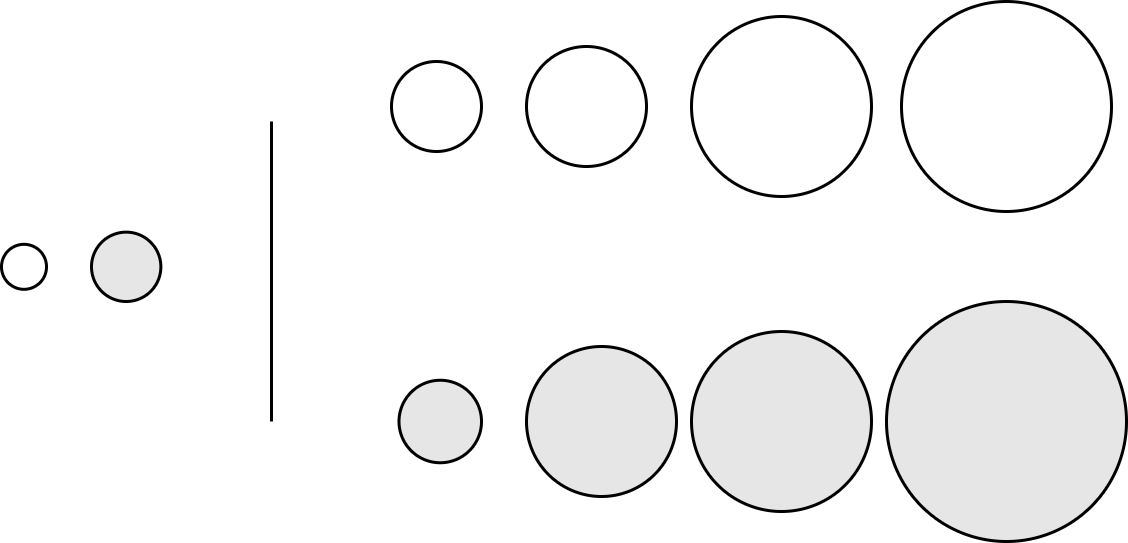
\includegraphics[scale=0.5]{img/merge2w}
 \caption{Merge}
 \label{fig:merge}
\end{figure}

\be
\begin{array}{rcl}
\textit{merge}\ [\ ]\ bs & = & bs \\
\textit{merge}\ as\ [\ ] & = & as \\
\textit{merge}\ (a \cons as)\ (b \cons bs) & = & \begin{cases}
  a < b: & a : \textit{merge}\ as\ (b \cons bs) \\
  \text{otherwise}: & b : \textit{merge}\ (a \cons as)\ bs
  \end{cases}
\end{array}
\label{eq:merge-sort-merge}
\ee

For array, we directly cut at the middle, recursively sort two halves, then merge:

\begin{algorithmic}[1]
\Procedure{Sort}{$A$}
  \State $n \gets |A|$
  \If{$n > 1$}
    \State $m \gets \lfloor \dfrac{n}{2} \rfloor$
    \State $X \gets$ \Call{Copy-Array}{$A[1...m]$}
    \State $Y \gets$ \Call{Copy-Array}{$A[m+1...n]$}
    \State \Call{Sort}{$X$}
    \State \Call{Sort}{$Y$}
    \State \Call{Merge}{$A, X, Y$}
  \EndIf
\EndProcedure
\end{algorithmic}

We allocated additional space of the same size as $A$ because \textproc{Merge} is not in-pace. We repeatedly compare elements from $X$ and $Y$, pick the less one to $A$. When either sub-array finishes, then add all the remaining to $A$.

\begin{algorithmic}[1]
\Procedure{Merge}{$A, X, Y$}
  \State $i \gets 1, j\gets 1, k\gets 1$
  \State $m \gets |X|, n \gets |Y|$
  \While{$i \leq m$ and $j \leq n$}
    \If{$X[i] < Y[j]$}
      \State $A[k] \gets X[i]$
      \State $i \gets i + 1$
    \Else
      \State $A[k] \gets Y[j]$
      \State $j \gets j + 1$
    \EndIf
    \State $k \gets k + 1$
  \EndWhile
  \While{$i \leq m$}
    \State $A[k] \gets X[i]$
    \State $k \gets k + 1$
    \State $i \gets i + 1$
  \EndWhile
  \While{$j \leq n$}
    \State $A[k] \gets Y[j]$
    \State $k \gets k + 1$
    \State $j \gets j + 1$
  \EndWhile
\EndProcedure
\end{algorithmic}

To simplify merge, we adjoin $\infty$ to $X$ and $Y$\footnote{$-\infty$ for descending order}.

\begin{algorithmic}[1]
\Procedure{Merge}{$A, X, Y$}
  \State \Call{Append}{$X, \infty$}
  \State \Call{Append}{$Y, \infty$}
  \State $i \gets 1, j\gets 1, n \gets |A|$
  \For{$k \gets$ from 1 to $n$}
    \If{$X[i] < Y[j]$}
      \State $A[k] \gets X[i]$
      \State $i \gets i + 1$
    \Else
      \State $A[k] \gets Y[j]$
      \State $j \gets j + 1$
    \EndIf
  \EndFor
\EndProcedure
\end{algorithmic}

\subsection{Performance}
\index{Merge Sort!Performance}

Merge sort takes two steps: partition and merge. It always halves the sequence. The binary partition tree is balanced as shown in \cref{fig:qsort-best}. Its height is $O(\lg n)$, so as the recursion depth. The merge happens at all levels, it compares elements one by one from each sorted sub-sequence, hence takes linear time. For sequence of length $n$, let $T(n)$ be the merge sort time, we have below recursive breakdown:

\be
T(n) = T(\dfrac{n}{2}) + T(\dfrac{n}{2}) + c n = 2 T(\dfrac{n}{2}) + c n
\ee

The time consists of three parts: sort the first and second halves, each takes $T(\dfrac{n}{2})$ time; and merge in $c n$ time, where $c$ is a constant. Solving this equation gives $T(n) = O(n \lg n)$. For space, varies implementation differ a lot. The basic merge sort allocates the space of the same size as the array in each recursion, copies elements and sorts, then release the space. It consumes the largest space of $O(n \lg n)$ when reaches to the deepest recursion.

\index{Merge Sort!Work area}
It's expensive to allocate/release space repeatedly\cite{Bentley}. We can pre-allocate a work area of the same size as $A$. Reuse it during recursion, and release it finally.

\begin{algorithmic}[1]
\Procedure{Sort}{A}
  \State $n \gets |A|$
  \State \textproc{Sort$'$}$(A$, \Call{Create-Array}{$n$}, $1, n)$
\EndProcedure
\Statex
\Procedure{Sort$'$}{$A, B, l, u$}
  \If{$u - l > 0$}
    \State $m \gets \lfloor \dfrac{l + u}{2} \rfloor$
    \State \Call{Sort$'$}{$A, B, l, m$}
    \State \Call{Sort$'$}{$A, B, m + 1, u$}
    \State \Call{Merge$'$}{$A, B, l, m, u$}
  \EndIf
\EndProcedure
\end{algorithmic}

We need update merge with the passed-in work area:

\begin{algorithmic}[1]
\Procedure{Merge$'$}{$A, B, l, m, u$}
  \State $i \gets l, j \gets m + 1, k \gets l$
  \While{$i \leq m$ and $j \leq u$}
    \If{$A[i] < A[j]$}
      \State $B[k] \gets A[i]$
      \State $i \gets i + 1$
    \Else
      \State $B[k] \gets A[j]$
      \State $j \gets j + 1$
    \EndIf
    \State $k \gets k + 1$
  \EndWhile
  \While{$i \leq m$}
    \State $B[k] \gets A[i]$
    \State $k \gets k + 1$
    \State $i \gets i + 1$
  \EndWhile
  \While{$j \leq u$}
    \State $B[k] \gets A[j]$
    \State $k \gets k + 1$
    \State $j \gets j + 1$
  \EndWhile
  \For{$i \gets$ from $l$ to $u$} \Comment{copy back}
    \State $A[i] \gets B[i]$
  \EndFor
\EndProcedure
\end{algorithmic}

This implementation reduces the space from $O(n \lg n)$ to $O(n)$, improves performance 20\% to 25\% for 100K numeric elements.

\subsection{In-place merge sort}
\index{Merge Sort!In-place merge sort}

To avoid additional space, consider how to reuse the array as the work area. As shown in \cref{fig:merge-in-place-naive}, sub-array $X$ and $Y$ are sorted. When merge in-place, the part before $l$ are merged and ordered. If $A[l] < A[m]$, move $l$ to right a step; otherwise ($A[l] \geq A[m]$), move $A[m]$ to the merged part before $l$. We need shift all elements in range $[l, m)$\footnote{range $[a, b)$ includes $a$, but excludes $b$.} to right a step.

\begin{figure}[htbp]
 \centering
      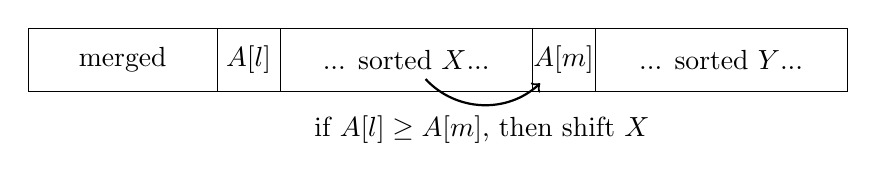
\begin{tikzpicture}[scale=0.8]
      \draw (0, 0) rectangle (3, 1) node [pos=.5] {merged}
            (3, 0) rectangle (4, 1) node [pos=.5] {$A[l]$}
            (4, 0) rectangle (8, 1) node (subA) [pos=.5] {... sorted $X$...}
            (8, 0) rectangle (9, 1) node (xsj) [pos=.5] {$A[m]$}
            (9, 0) rectangle (13, 1) node [pos=.5] {... sorted $Y$...};
      \draw[thick, ->] (subA) edge [bend right=45] node [below] {if $A[l] \geq A[m]$, then shift $X$} (xsj);
      \end{tikzpicture}
 \caption{In-place shift and merge}
 \label{fig:merge-in-place-naive}
\end{figure}

\begin{algorithmic}[1]
\Procedure{Merge}{$A, l, m, u$}
  \While{$l \leq m \land m \leq u$}
    \If{$A[l] < A[m]$}
      \State $l \gets l + 1$
    \Else
      \State $x \gets A[m]$
      \For{$i \gets m $ down-to $l+1$} \Comment{Shift}
        \State $A[i] \gets A[i-1]$
      \EndFor
      \State $A[l] \gets x$
    \EndIf
  \EndWhile
\EndProcedure
\end{algorithmic}

\index{Merge Sort!Work area}
However, it downgrades to $O(n^2)$ time because array shift takes linear time ($O(|X|$). When sort sub-array, we want to reuse the remaining part as the work area, and must avoid overwriting any elements. We compare elements from sorted sub-array $X$ and $Y$, pick the less one and store it in the work area. However, we need exchange the element out to free up the cell. After merge, $X$ and $Y$ together store the content of the original work area, as shown in \cref{fig:merge-workarea}.

\begin{figure}[htbp]
 \centering
      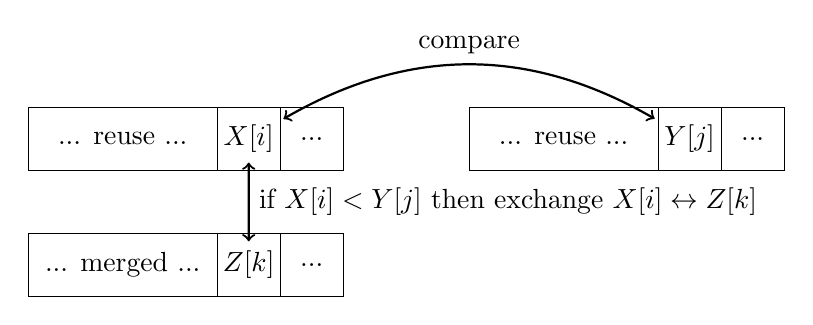
\begin{tikzpicture}[scale=0.8]
      \draw (0, 2) rectangle (3, 3) node [pos=.5] {... reuse ...}
            (3, 2) rectangle (4, 3) node (ai) [pos=.5] {$X[i]$}
            (4, 2) rectangle (5, 3) node [pos=.5] {...}
            (7, 2) rectangle (10, 3) node [pos=.5] {... reuse ...}
            (10, 2) rectangle (11, 3) node (bj) [pos=.5] {$Y[j]$}
            (11, 2) rectangle (12, 3) node [pos=.5] {...}
            (0, 0) rectangle (3, 1) node [pos=.5] {... merged ...}
            (3, 0) rectangle (4, 1) node (ck) [pos=.5] {$Z[k]$}
            (4, 0) rectangle (5, 1) node [pos=.5] {...};
      \draw[thick, <->] (ai) edge [bend left] node [above] {compare} (bj)
                        (ai) edge node [right] {if $X[i] < Y[j]$ then exchange $X[i] \leftrightarrow Z[k]$} (ck);
      \end{tikzpicture}
 \caption{Merge and swap}
 \label{fig:merge-workarea}
\end{figure}

The sorted $X$, $Y$, and the work area $Z$ are all sub-arrays. We pass the start, end positions of $X$ and $Y$ as ranges $[i, m)$, $[j, n)$. The work area starts from $k$.

\begin{algorithmic}[1]
\Procedure{Merge}{$A, [i, m), [j, n), k$}
  \While{$i < m$ and $j < n$}
    \If{$A[i] < A[j]$}
      \State \textproc{Exchange} $A[k] \leftrightarrow A[i]$
      \State $i \gets i + 1$
    \Else
      \State \textproc{Exchange} $A[k] \leftrightarrow A[j]$
      \State $j \gets j + 1$
    \EndIf
    \State $k \gets k + 1$
  \EndWhile
  \While{$i < m$}
    \State \textproc{Exchange} $A[k] \leftrightarrow A[i]$
    \State $i \gets i + 1$
    \State $k \gets k + 1$
  \EndWhile
  \While{$j < m$}
    \State \textproc{Exchange} $A[k] \leftrightarrow A[j]$
    \State $j \gets j + 1$
    \State $k \gets k + 1$
  \EndWhile
\EndProcedure
\end{algorithmic}

The work area has two properties: 1) It has sufficient size to hold the elements swapped in; 2) It can overlap with either sorted sub-arrays, but must not overwrite any unmerged elements. One idea is to use half array as the work area to sort the other half, as shown in \cref{fig:merge-in-place-start}.

\begin{figure}[htbp]
 \centering
      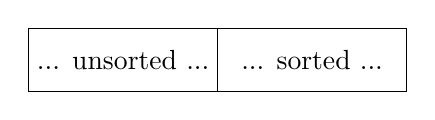
\begin{tikzpicture}[scale=0.8]
      \draw (0, 0) rectangle (3, 1) node [pos=.5] {... unsorted ...}
            (3, 0) rectangle (6, 1) node [pos=.5] {... sorted ...};
      \end{tikzpicture} \\
 \caption{Merge and sort half array}
 \label{fig:merge-in-place-start}
\end{figure}

We next sort further half of the work area (remaining $\dfrac{1}{4}$), as shown in \cref{fig:merge-in-place-quater}. We must merge $X$ ($\dfrac{1}{2}$ array) and $Y$ ($\dfrac{1}{4}$ array) later sometime. However, the work area can only hold $\dfrac{1}{4}$ array, insufficient for the size of $X + Y$.

\begin{figure}[htbp]
 \centering
 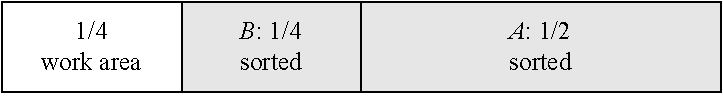
\includegraphics[scale=0.8]{img/workarea-1}
 \caption{Work area can't support merge $X$ and $Y$.}
 \label{fig:merge-in-place-quater}
\end{figure}

The second property gives a way out: arrange the work area overlapped with either sub-array, and only override the merged part. We first sort the second 1/2 of the work area, as the result, swap $Y$ to the first 1/2, the new work area is between $X$ and $Y$, as shown in the upper of \cref{fig:merge-in-place-setup}. The work area is overlapped with $X$\cite{msort-in-place}. Consider two extremes:

\begin{figure}[htbp]
 \centering
 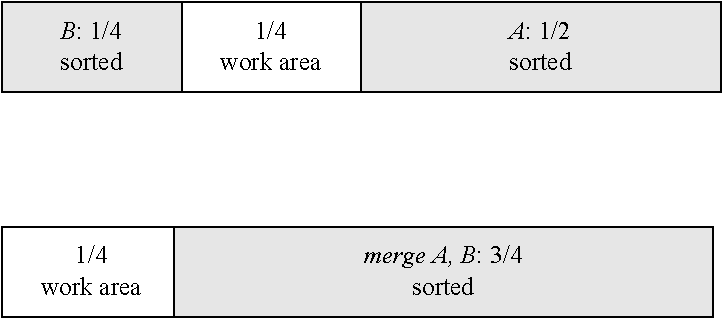
\includegraphics[scale=0.8]{img/workarea-2}
 \caption{Merge $X$ and $Y$ with the work area.}
 \label{fig:merge-in-place-setup}
\end{figure}

\begin{enumerate}
\item $y < x$, for all $y$ in $Y$, $x$ in $X$. After merge, contents of $Y$ and the work area are swapped (the size of $Y$ equals to the work area);
\item $x < y$, for all $y$ in $Y$, $x$ in $X$. During merge, we repeatedly swap content of $X$ and the work area. After half of $X$ is swapped, we start overriding $X$. Fortunately, we only override the merged content. The right boundary of work area keep extending to the 3/4 of the array. After that, we start swapping the content of $Y$ and the work area. Finally, the work area moves to the left side of the array, as shown in the bottom of \cref{fig:merge-in-place-setup}.
\end{enumerate}

The other cases are between the above two extremes. The work area finally moves to the first 1/4 of the array. Repeat this, we always sort the second 1/2 of the work area, swap the result to the first 1/2, and keep the work area in the middle. We halve the work area every time $\dfrac{1}{2}, \dfrac{1}{4}, \dfrac{1}{8}, ...$ of the array, terminate when there is only one element left. Alternatively, we can fallback to insert sort for the last few elements.

\begin{algorithmic}[1]
\Procedure{Sort}{$A, l, u$}
  \If{$u - l > 0$}
    \State $m \gets \lfloor \dfrac{l + u}{2} \rfloor$
    \State $w \gets l + u - m$
    \State \Call{Sort'}{$A, l, m, w$} \Comment{sort half}
    \While{$w - l > 1$}
      \State $u' \gets w$
      \State $w \gets \lceil \dfrac{l + u'}{2} \rceil$ \Comment{halve the work area}
      \State \Call{Sort'}{$A, w, u', l$} \Comment{sort the remaining half}
      \State \Call{Merge}{$A, [l, l + u' - w], [u', u], w$}
    \EndWhile
    \For{$i \gets w$ down-to $l$} \Comment{Switch to insert sort}
      \State $j \gets i$
      \While{$j \leq u$ and $A[j] < A[j-1]$}
        \State \textproc{Exchange} $A[j] \leftrightarrow A[j-1]$
        \State $j \gets j + 1$
      \EndWhile
    \EndFor
  \EndIf
\EndProcedure
\end{algorithmic}

We round up the work area to ensure sufficient size, then pass the range and work area to \textproc{Merge}. We next update \textproc{Sort'}, which calls \textproc{Sort} to swap the work area and the merged part.

\begin{algorithmic}[1]
\Procedure{Sort'}{$A, l, u, w$}
  \If{$u - l > 0$}
    \State $m \gets \lfloor \dfrac{l + u}{2} \rfloor$
    \State \Call{Sort}{$A, l, m$}
    \State \Call{Sort}{$A, m+1, u$}
    \State \Call{Merge}{$A, [l, m), [m+1, u), w$}
  \Else \Comment{Swap elements to the work area}
    \While{$l \leq u$}
      \State \textproc{Exchange} $A[l] \leftrightarrow A[w]$
      \State $l \gets l + 1$
      \State $w \gets w + 1$
    \EndWhile
  \EndIf
\EndProcedure
\end{algorithmic}

This implementation needn't shift sub-array, it keeps reducing the unordered part: $\dfrac{n}{2}, \dfrac{n}{4}, \dfrac{n}{8}, ...$, completes in $O(\lg n)$ steps. Every step sorts half of the remaining, then merge in linear time. Let the time to sort $n$ elements be $T(n)$, we have the following recursive result:

\be
T(n) = T(\frac{n}{2}) + c \frac{n}{2} + T(\frac{n}{4}) + c \frac{3n}{4} + T(\frac{n}{8}) + c \frac{7n}{8} + ...
\label{eq:in-place-sort-time}
\ee

For half elements, the time is:

\be
T(\frac{n}{2}) = T(\frac{n}{4}) + c \frac{n}{4} + T(\frac{n}{8}) + c \frac{3n}{8} + T(\frac{n}{16}) + c \frac{7n}{16} + ...
\label{eq:in-place-sort-time-half}
\ee

Subtract \cref{eq:in-place-sort-time} and \cref{eq:in-place-sort-time-half}:

\[
T(n) - T(\frac{n}{2}) = T(\frac{n}{2}) + c n (\frac{1}{2} + \frac{1}{2} + ... )
\]

It adds $\dfrac{1}{2}$ with total $\lg n$ times, hence:

\[
T(n) = 2 T(\frac{n}{2}) + \frac{c}{2} n \lg n
\]

Apply telescope method, (or master theorem) gives the result $O(n \lg^2 n)$.

\subsection{Nature merge sort}
\index{Merge Sort!Nature merge sort}

\begin{figure}[htbp]
 \centering
 \includegraphics[scale=0.25]{img/burn-candle-2-ends}
 \caption{Burn from both ends}
 \label{fig:burn-candle}
\end{figure}

Knuth gives another implementation, called {\em nature merge sort}. It likes burning a candle from both ends\cite{TAOCP}. For any sequence, one can always find an ordered segment from any position. Particularly, we can find such a segment from left end as shown in below table.

\btab{l}
\underline{15}, 0, 4, 3, 5, 2, 7, 1, 12, 14, 13, 8, 9, 6, 10, 11 \\
\underline{8, 12, 14}, 0, 1, 4, 11, 2, 3, 5, 9, 13, 10, 6, 15, 7 \\
\underline{0, 1, 2, 3, 4, 5, 6, 7, 8, 9, 10, 11, 12, 13, 14, 15 } \\
\etab

The first row is the extreme case of a singleton segment; the third row is the other extreme that the segment extends to the right end, the whole sequence is ordered. Symmetrically, we can always find ordered segment from right end, then merge the two sorted segments, one from left, another from right. The advantage is to re-use the nature ordered sub-sequences for partition.

\begin{figure}[htbp]
 \centering
 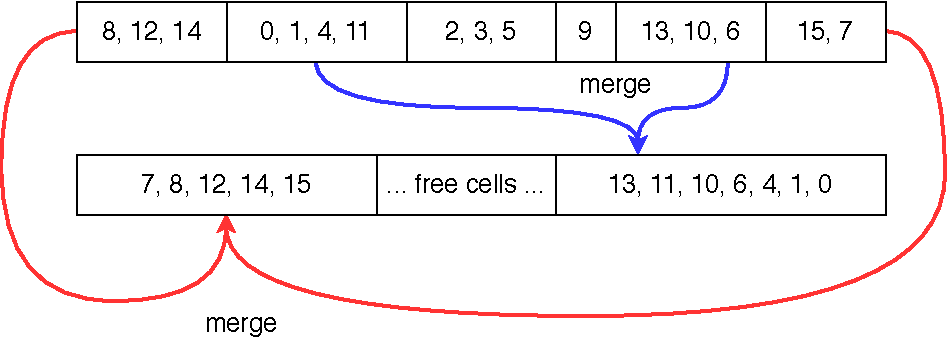
\includegraphics[scale=0.7]{img/nature-merge-sort}
 \caption{Nature merge sort}
 \label{fig:nature-merge-sort}
\end{figure}

As shown in \cref{fig:nature-merge-sort}, scan from both ends, find the two longest ordered segments respectively. Then merge them to the left of the work area. Next, restart to scan from left and right to center. This time, merge the two segments from the right to left of the work area. We switch the merge direction right/left in-turns. After scanning all elements and merge them to the work area, swap the original array and the work area, then start a new round of bi-directional scan and merge. Terminate when the ordered segment extends to cover the whole array. This implementation processes the array from both directions based on nature ordering, called {\em nature two-way merge sort}. As shown in \cref{fig:nature-msort-invariant}, elements before $a$ and after $d$ are scanned. We span the ordered segment $[a, b)$ to right, meanwhile, span $[c, d)$ to left. For the work area, elements before $f$ and after $f$ are merged (consist of multiple sub-sequences). In odd rounds, we merge $[a, b)$ and $[c, d)$ from $f$ to right; in even rounds, merge from $r$ to left.

\captionsetup[subfigure]{labelformat=empty, margin=10pt}
\begin{figure}[htbp]
 \centering
   \subcaptionbox{}{
      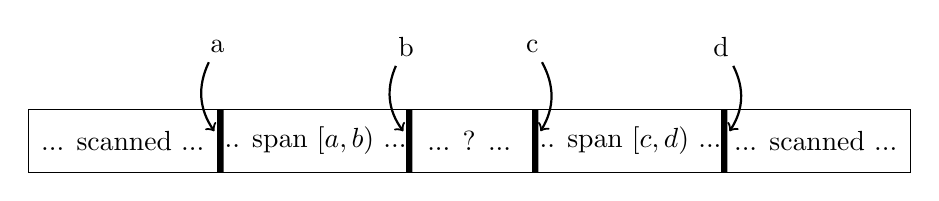
\begin{tikzpicture}[scale=0.8]
      \draw (0, 0) rectangle (3, 1) node [pos=.5] {... scanned ...}
            (3, 0) rectangle (6, 1) node [pos=.5] {... span $[a, b)$ ...}
            (6, 0) rectangle (8, 1) node [pos=.5] {... ? ...}
            (8, 0) rectangle (11, 1) node [pos=.5] {... span $[c, d)$ ...}
            (11, 0) rectangle (14, 1) node [pos=.5] {... scanned ...};
      \fill [black] (3, 0) rectangle (3.1, 1) node (abar) [pos=.5] {}
                    (6, 0) rectangle (6.1, 1) node (bbar) [pos=.5] {}
                    (8, 0) rectangle (8.1, 1) node (cbar) [pos=.5] {}
                    (11, 0) rectangle (11.1, 1) node (dbar) [pos=.5] {};
      \draw (3, 2) node (a) {a}
            (6, 2) node (b) {b}
            (8, 2) node (c) {c}
            (11, 2) node (d) {d};
      \draw[thick, ->] (a) edge [bend right] (abar)
                       (b) edge [bend right] (bbar)
                       (c) edge [bend left] (cbar)
                       (d) edge [bend left] (dbar);
      \end{tikzpicture}} \\
    \subcaptionbox{}{
      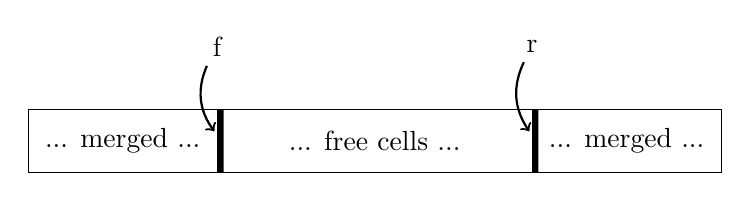
\begin{tikzpicture}[scale=0.8]
      \draw (0, 0) rectangle (3, 1) node [pos=.5] {... merged ...}
            (3, 0) rectangle (8, 1) node [pos=.5] {... free cells ...}
            (8, 0) rectangle (11, 1) node [pos=.5] {... merged ...};
      \fill [black] (3, 0) rectangle (3.1, 1) node (fbar) [pos=.5] {}
                    (8, 0) rectangle (8.1, 1) node (rbar) [pos=.5] {};
      \draw (3, 2) node (f) {f}
            (8, 2) node (r) {r};
      \draw[thick, ->] (f) edge [bend right] (fbar)
                       (r) edge [bend right] (rbar);
      \end{tikzpicture}} \\
 \caption{A status of nature merge sort}
 \label{fig:nature-msort-invariant}
\end{figure}
\captionsetup[subfigure]{labelformat=parens}

When start, we allocate a work area of the same size as the array. $a$, $b$ point to the left side, $c$, $d$ point to the right side. $f$, $r$ point to the two sides of the work area respectively.

\begin{algorithmic}[1]
\Function{Sort}{$A$}
  \If{$|A| > 1$}
    \State $n \gets |A|$
    \State $B \gets$ \Call{Create-Array}{$n$}  \Comment{the work area}
    \Loop
      \State $[a, b) \gets [1, 1)$
      \State $[c, d) \gets [n+1, n+1)$
      \State $f \gets 1, r \gets n$ \Comment{front, rear of the work area}
      \State $t \gets 1$            \Comment{even/odd round}
      \While{$b < c$}               \Comment{elements yet to scan}
        \Repeat \Comment{Span $[a, b)$}
          \State $b \gets b + 1$
        \Until{$b \geq c \lor A[b] < A[b-1]$}

        \Repeat \Comment{Span $[c, d)$}
          \State $c \gets c - 1$
        \Until{$c \leq b \lor A[c-1] < A[c]$}

        \If{$c < b$} \Comment{Avoid overlap}
          \State $c \gets b$
        \EndIf

        \If{$b - a \geq n$} \Comment{Terminate if $[a, b)$ spans the whole array}
          \State \Return $A$
        \EndIf

        \If{$t$ is odd} \Comment{merge to front}
          \State $f \gets$ \Call{Merge}{$A, [a, b), [c, d), B, f, 1$}
        \Else \Comment{merge to rear}
          \State $r \gets$ \Call{Merge}{$A, [a, b), [c, d), B, r, -1$}
        \EndIf
        \State $a \gets b, d \gets c$
        \State $t \gets t + 1$
      \EndWhile
      \State \textproc{Exchange} $A \leftrightarrow B$ \Comment{Switch work area}
    \EndLoop
  \EndIf
  \State \Return $A$
\EndFunction
\end{algorithmic}

We need pass the merge direction in:

\begin{algorithmic}[1]
\Function{Merge}{$A, [a, b), [c, d), B, w, \Delta$}
  \While{$a < b$ and $c < d$}
    \If{$A[a] < A[d-1]$}
      \State $B[w] \gets A[a]$
      \State $a \gets a + 1$
    \Else
      \State $B[w] \gets A[d-1]$
      \State $d \gets d - 1$
    \EndIf
    \State $w \gets w + \Delta$
  \EndWhile
  \While{$a < b$}
    \State $B[w] \gets A[a]$
    \State $a \gets a + 1$
    \State $w \gets w + \Delta$
  \EndWhile
  \While{$c < d$}
    \State $B[w] \gets A[d-1]$
    \State $d \gets d - 1$
    \State $w \gets w + \Delta$
  \EndWhile
  \State \Return $w$
\EndFunction
\end{algorithmic}

The performance does not depend on how ordered the elements are. In the `worst' case, the ordered sub-sequences are all singleton. After merge, the length of the new ordered sub-sequences are at least 2. Suppose we still encounter the `worst' case in the second round, the merged sub-sequences have length at least 4, ... every round doubles the sub-sequence length, hence we need at most $O(\lg n)$ rounds. Because we scan all elements every round, the total time is bound to $O(n \lg n)$. For list, we can't scan from tail back easily as array. A list consists multiple ordered sub-lists, we merge them in pairs. It halves the sub-lists every round, and finally builds the sorted result. Define this as (Curried form):

\be
sort = sort' \circ group
\ee

Where $group$ breaks the list into ordered sub-lists:

\be
\begin{array}{rcl}
\textit{group}\ [\ ] & = & [[\ ]] \\
\textit{group}\ [x] & = & [[x]] \\
\textit{group}\ (x \cons y \cons xs) & = & \begin{cases}
  x < y: & (x \cons g) \cons gs, \text{where}\ (g \cons gs) = \textit{group}\ (y \cons xs) \\
  \text{otherwise}: & [x] \cons g \cons gs \\
\end{cases}
\end{array}
\ee

\be
\begin{array}{rcl}
\textit{sort}'\ [\ ] & = & [\ ] \\
\textit{sort}'\ [g] & = & g \\
\textit{sort}'\ gs & = & \textit{sort}'\ (\textit{mergePairs}\ gs) \\
\end{array}
\ee

Where:

\be
\begin{array}{rcl}
\textit{mergePairs}\ (g_1 \cons g_2 \cons gs) & = & merge\ g_1\ g_2 : \textit{mergePairs}\ gs \\
\textit{mergePairs}\ gs & = & gs
\end{array}
\ee

\begin{Exercise}\label{ex:multi-merge}
\Question{One defines $\textit{sort}' = foldr\ merge\ [\ ]$. Is the performance same as the pairwise merge ($mergePairs$)? If yes, prove it; if not, which one is faster?}
\end{Exercise}

\begin{Answer}[ref = {ex:multi-merge}]
\Question{The pairwise merge is faster. This problem is essentially to merge $k$ ordered sequences. Assume the average length of the $k$ sequences is $n$ for simplification. When merge with fold, we first merge $s_1$ and the empty sequence $merge([\ ], s_1) = [\ ] \oplus s_1$, then merge $s_2$ to get $[\ ] \oplus s_1 \oplus s_2$, then merge $s_3$ to get $[\ ] \oplus s_1 \oplus s_2 \oplus s_3$, ..., the total complexity is $O(n + 2n + 3n + 4n + ... + kn) = O(n\dfrac{k(k+1)}{2}) = O(nk^2)$. While for pairwise merging, the first round is to merge $s_1 \oplus s_2$, $s_3 \oplus s_4$, ..., takes $O(kn)$ time in total; the next round is to merge $(s_1 \oplus s_2) \oplus (s_3 \oplus s_4)$, ..., taking $O(kn)$ time too. There are total $lg k$ rounds, hence the total complexity is $O(nk \lg k)$. Therefore the pairwise merge performs better.

We can also merge with a min-heap of size $k$. Store the minimum elements from each sequence in the heap, keep popping the overall minimum one, and replace it with the next element in that sequence. The complexity is $O(nk \lg k)$ too.
}
\end{Answer}

\subsection{Bottom-up merge sort}
\index{Merge Sort!Bottom-up merge sort}

We can develop the bottom-up merge sort from the above performance analysis. First wrap all elements as $n$ singletons. Then merge them in pairs to obtain $\frac{n}{2}$ ordered sub-lists of length 2; If $n$ is odd, there remains a single list. Repeat this paired merge to sort all. Knuth calls it `straight two-way merge sort'\cite{TAOCP}, as shown in \cref{fig:bottom-up-msort}.

\begin{figure}[htbp]
 \centering
 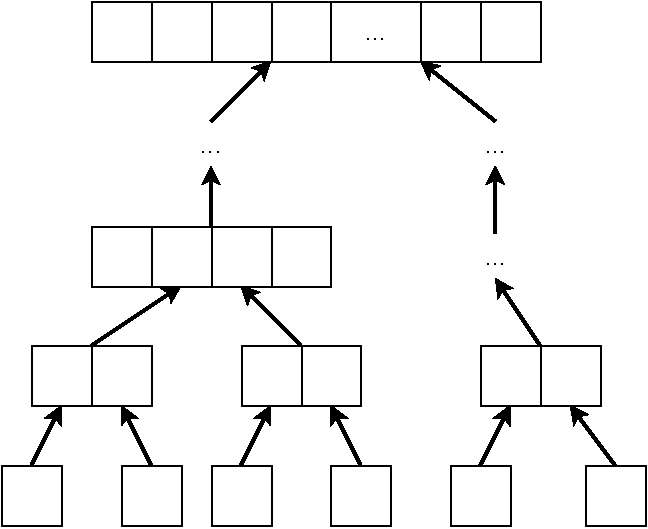
\includegraphics[scale=0.6]{img/bottom-up-msort}
 \caption{Bottom-up merge sort}
 \label{fig:bottom-up-msort}
\end{figure}

We needn't partition the list. When start, convert $[x_1, x_2, ..., x_n]$ to $[[x_1], [x_2], ..., [x_n]]$, then apply paired merge:

\be
sort = sort' \circ map (x \mapsto [x])
\ee

We reuse the \textit{mergePairs} defined for nature merge sort, terminates when consolidates to one list\cite{okasaki-book}. The bottom up sort is similar to the nature merge sort, different only in partition method. It can be deduced from nature merge sort as a special case (the `worst' case). Nature merge sort always spans the ordered sub-sequence as long as possible; while the bottom up merge sort only spans the length to 1. From the tail recursive implementation, we can eliminate the recursion and convert it to iterative loops.

\begin{algorithmic}[1]
\Function{Sort}{$A$}
  \State $n \gets |A|$
  \State $B \gets $ \Call{Create-Array}{$n$}
  \For{$i$ from 1 to $n$}
    \State $B[i] = [A[i]]$
  \EndFor
  \While{$n > 1$}
    \For{$i \gets $ from $1$ to $\lfloor \dfrac{n}{2} \rfloor$}
      \State $B[i] \gets$ \Call{Merge}{$B[2i -1], B[2i]$}
    \EndFor
    \If{\Call{Odd}{$n$}}
      \State $B[\lceil \dfrac{n}{2} \rceil] \gets B[n]$
    \EndIf
    \State $n \gets \lceil \dfrac{n}{2} \rceil$
  \EndWhile
  \If{$B = [\ ]$}
    \State \Return $[\ ]$
  \EndIf
  \State \Return $B[1]$
\EndFunction
\end{algorithmic}

\begin{Exercise}\label{ex:pairwise-fold}
\Question{Define the generic pairwise fold $foldp$, and use it to implement the bottom-up merge sort.}
\end{Exercise}

\begin{Answer}[ref = {ex:pairwise-fold}]
\Question{Define the generic pairwise fold $foldp$, and use it to implement the bottom-up merge sort.

It's sufficient the binary combination function $f$ be associative, i.e., $f(f(x, y), z) = f(x, f(y, z))$. Let the unit of $f$ be $z$, define the pairwise fold as:

\begin{Haskell}
foldp f z [] = z
foldp f z [x] = f x z
foldp f z xs = foldp f z (pairs xs) where
  pairs (x:y:ys) = (f x y) : pairs ys
  pairs ys = ys
\end{Haskell}

For example, we can define $sum = foldp\ (+)\ 0$, and the bottom-up merge sort is defined as\footnote{\lstinline{(:[])} is equivalent to $x\ xs \mapsto [x] \cons xs$.}:
\begin{Haskell}
sort = foldp merge [] . map (:[])
\end{Haskell}
}
\end{Answer}

\section{Parallelism}
\index{Parallel merge sort} \index{Parallel quick sort}

In quick sort implementation, we can parallel sorting the two sub-sequences after partition. Similarly, to parallel merge sort. Actually, we don't limit by two concurrent tasks, but divide into $p$ sub-sequences, where $p$ is the number of processors. Ideally, if we can achieve sorting in $T'$ time with parallelism, where $O(n \lg n) = p T'$, we say it's {\em linear speed up}, and the algorithm is parallel optimal. However, it is not parallel optimal by choosing $p - 1$ pivots, and partition the sequence into $p$ parts for quick sort. The bottleneck happens in the divide phase, that can only achieve in $O(n)$ time. While, the bottleneck is the merge phase for parallel merge sort. Both need specific design to speed up. Basically, the divide and conquer nature makes merge sort and quick sort relative easy for parallelism. Richard Cole developed parallel merge sort achieved $O(\lg n)$ performance with $n$ processors in 1986\cite{para-msort}. Parallelism is a big and complex topic out of the elementary scope\cite{para-msort}\cite{para-qsort}.

\section{Summary}

This chapter gives two popular divide and conquer sort algorithms: quick sort and merge sort. Both achieve the best performance of $O(n \lg n)$ for comparison based sort. Sedgewick quotes quick sort as the greatest algorithm developed in the 20th century. Many programming environments provide sort tool based on it. Merge sort is a powerful tool when handling sequence of complex entities, or not persisted in array\footnote{In practice, most are kind of hybrid sort, for example, fallback to insert sort for small sequence.}. Quick sort performs well in most cases with fewer swaps than other methods. However, swap is not suitable for linked-list, while merge sort is. It costs constant space and the performance is guaranteed for all cases. Quick sort has advantage for vector storage like arrays, because it needn't extra work area and can sort in-place. This is a valuable feature particularly in embedded system where memory is limited. In-place merging is till an active research area.

We can consider quick sort as the optimized tree sort. Similarly, we can also deduce merge sort from tree sort\cite{sort-deriving}. People categorize sort algorithms in different ways\cite{TAOCP}, for example, from the perspective of partition and merge\cite{algo-fp}. Quick sort is easy to merge, because all the elements in one sub-sequence are not greater than the other. Merge is equivalent to concatenation. While merge sort is easy to partition no matter cut at the middle, even-odd split, nature split, or bottom up split. It's difficult to achieve perfect partition in quick sort, we can't completely avoid the worst case no matter with median-of-three pivot, random quick sort, or ternary quick sort.

As of this chapter, we've seen the elementary sort algorithms, including insert sort, tree sort, selection sort, heap sort, quick sort, and merge sort. Sort is an important domain in computer algorithm design. People are facing the `big data' challenge when I write this chapter. It becomes routine to sort hundreds of Gigabytes with limited resources and time.

\begin{Exercise}\label{ex:bst-merge}
\Question{Build a binary search tree from a sequence using the idea of merge sort.}
\end{Exercise}

\begin{Answer}[ref={ex:bst-merge}]
\Question{Build a binary search tree from a sequence using the idea of merge sort.

\vspace{3mm}
We can build the binary search tree either top-down or bottom-up. For top-down, halve the list to two, recursively build two trees respectively then merge; for bottom-up, wrap each element to a singleton leaf, then pair-wise merge trees repeatedly to the final result. Both approaches depend on the tree merge, let us define it\footnote{For the standalone problem of binary search tree merge, we can flatten the trees to two arrays (or lists through in-order traverse), then apply $merge$ (see \cref{eq:merge-sort-merge}), and rebuild the tree with the middle element as the root.}. If either tree is empty, the merge result is the other; otherwise, let the two trees be $(A, x, B)$ and $(C, y, D)$, if $x < y$, use $y$ to partition $B$ to two trees $B_y$ and $B^y$, where $B_y$ has all elements $\{b < y\}$, and $B_y$ has the rest $\{b \geq y\}$; use $x$ to partition $C$ to $C_x$ and $C^x$. We then form the merge result as:

\[
(A, x, B) \oplus (C, y, D) = ((A \oplus C_x, x, B_y \oplus C^x), y, D \oplus B^y)
\]

Where `$\oplus$' means tree merge. Symmetrically, when $x \geq y$, we partition $A$ and $D$. Below example program implements tree \textit{partition} and \textit{merge}. It uses \textit{foldp} defined in \cref{ex:pairwise-fold}.

\begin{Haskell}
toTree :: (Ord a) => [a] -> Tree a
toTree = foldp merge Empty . map leaf

partition x Empty = (Empty, Empty)
partition x (Node a y b)
  | x < y = let (a1, a2) = partition x a in (a1, Node a2 y b)
  | otherwise = let (b1, b2) = partition x b in (Node a y b1, b2)

merge Empty t = t
merge t Empty = t
merge (Node a x b) (Node c y d)
  | x < y = let
      (b1, b2) = partition y b
      (c1, c2) = partition x c
      in Node (Node (merge a c1) x (merge b1 c2)) y (merge d b2)
  | otherwise = let
      (a1, a2) = partition y a
      (d1, d2) = partition x d
      in Node (merge a1 c) y (Node (merge a2 d1) x (merge b d2))
\end{Haskell}
}
\end{Answer}

\section{Appendix: Example programs}

In-place partition:

\begin{lstlisting}[language = Bourbaki]
Int partition([K] xs, Int l, Int u) {
    for (Int pivot = l, Int r = l + 1; r < u; r = r + 1) {
        if xs[pivot] >= xs[r] {
            l = l + 1
            swap(xs[l], xs[r])
        }
    }
    swap(xs[pivot], xs[l])
    return l + 1
}

Void sort([K] xs, Int l, Int u) {
    if l < u {
        Int m = partition(xs, l, u)
        sort(xs, l, m - 1)
        sort(xs, m, u)
    }
}
\end{lstlisting}

Bi-directional scan:

\begin{lstlisting}[language = Bourbaki]
Void sort([K] xs, Int l, Int u) {
    if l < u - 1 {
        Int pivot = l, Int i = l, Int j = u
        loop {
            while i < u and xs[i] < xs[pivot] {
                i = i + 1
            }
            while j >=l and xs[pivot] < xs[j] {
                j = j - 1
            }
            if j < i then break
            swap(xs[i], xs[j])
        }
        swap(xs[pivot], xs[j])
        sort(xs, l, j)
        sort(xs, i, u)
    }
}
\end{lstlisting}

Merge sort:

\begin{lstlisting}[language = Bourbaki]
[K] sort([K] xs) {
    Int n = length(xs)
    if n > 1 {
        var ys = sort(xs[0 ... n/2 - 1])
        var zs = sort(xs[n/2 ...])
        xs = merge(xs, ys, zs)
    }
    return xs
}

[K] merge([K] xs, [K] ys, [K] zs) {
    Int i = 0
    while ys != [] and zs != [] {
        xs[i] = if ys[0] < zs[0] then pop(ys) else pop(zs)
        i = i + 1
    }
    xs[i...] = if ys !=[] then ys else zs
    return xs
}
\end{lstlisting}

Merge sort with work area:

\lstset{language=C}
\begin{lstlisting}[language = Bourbaki]
Void sort([K] xs) = msort(xs, copy(xs), 0, length(xs))

Void msort([K] xs, [K] ys, Int l, Int u) {
    if (u - l > 1) {
        Int m = l + (u - l) / 2
        msort(xs, ys, l, m)
        msort(xs, ys, m, u)
        merge(xs, ys, l, m, u)
    }
}

Void merge([K] xs, [K] ys, Int l, Int m, Int u) {
    Int i = l, Int k = l; Int j = m
    while i < m and j < u {
        ys[k++] = if xs[i] < xs[j] then xs[i++] else xs[j++]
    }
    while i < m {
        ys[k++] = xs[i++]
    }
    while j < u {
        ys[k++] = xs[j++]
    }
    while l < u {
        xs[l] = ys[l]
        l++
    }
}
\end{lstlisting}

In-place merge sort:

\begin{lstlisting}[language = Bourbaki]
Void merge([K] xs, (Int i, Int m), (Int j, Int n), Int w) {
    while i < m and j < n {
        swap(xs, w++, if xs[i] < xs[j] then i++ else j++)
    }
    while i < m {
        swap(xs, w++, i++)
    }
    while j < n {
        swap(xs, w++, j++)
    }
}

Void wsort([K] xs, (Int l, Int u), Int w) {
    if u - l > 1 {
        Int m = l + (u - l) / 2
        imsort(xs, l, m)
        imsort(xs, m, u)
        merge(xs, (l, m), (m, u), w)
    }
    else {
        while l < u { swap(xs, l++, w++) }
    }
}

Void imsort([K] xs, Int l, Int u) {
    if u - l > 1 {
        Int m = l + (u - l) / 2
        Int w = l + u - m
        wsort(xs, l, m, w)
        while w - l > 2 {
            Int n = w
            w = l + (n - l + 1) / 2;
            wsort(xs, w, n, l);
            merge(xs, (l, l + n - w), (n, u), w);
        }
        for Int n = w; n > l; --n {
            for Int m = n; m < u and xs[m] < xs[m-1]; m++ {
                swap(xs, m, m - 1)
            }
        }
    }
}
\end{lstlisting}

Iterative bottom up merge sort:

\begin{lstlisting}[language = Bourbaki]
[K] sort([K] xs) {
    var ys = [[x] | x in xs]
    while length(ys) > 1 {
        ys += merge(pop(ys), pop(ys))
    }
    return if ys == [] then [] else pop(ys)
}

[K] merge([K] xs, [K] ys) {
    [K] zs = []
    while xs != [] and ys !=[] {
        zs += if xs[0] < ys[0] then pop(xs) else pop(ys)
    }
    return zs ++ (if xs !=[] then xs else ys)
}
\end{lstlisting}

\ifx\wholebook\relax\else
\section{Answers}
\shipoutAnswer

\begin{thebibliography}{99}

\bibitem{TAOCP}
Donald E. Knuth. ``The Art of Computer Programming, Volume 3: Sorting and Searching (2nd Edition)''. Addison-Wesley Professional; 2 edition (May 4, 1998) ISBN-10: 0201896850 ISBN-13: 978-0201896855

\bibitem{CLRS}
Thomas H. Cormen, Charles E. Leiserson, Ronald L. Rivest and Clifford Stein.
``Introduction to Algorithms, Second Edition''. ISBN:0262032937. The MIT Press. 2001

\bibitem{qsort-impl}
Robert Sedgewick. ``Implementing quick sort programs''. Communication of ACM. Volume 21, Number 10. 1978. pp.847 - 857.

\bibitem{Bentley}
Jon Bentley. ``Programming pearls, Second Edition''. Addison-Wesley Professional; 1999. ISBN-13: 978-0201657883

\bibitem{3-way-part}
Jon Bentley, Douglas McIlroy. ``Engineering a sort function''. Software Practice and experience VOL. 23(11), 1249-1265 1993.

\bibitem{opt-qs}
Robert Sedgewick, Jon Bentley. ``Quicksort is optimal''. \url{http://www.cs.princeton.edu/~rs/talks/QuicksortIsOptimal.pdf}

\bibitem{fp-pearls}
Richard Bird. ``Pearls of functional algorithm design''. Cambridge University Press. 2010. ISBN, 1139490605, 9781139490603

\bibitem{algo-fp}
Fethi Rabhi, Guy Lapalme. ``Algorithms: a functional programming approach''. Second edition. Addison-Wesley, 1999. ISBN: 0201-59604-0

\bibitem{slpj}
Simon Peyton Jones. ``The Implementation of functional programming languages''. Prentice-Hall International, 1987. ISBN: 0-13-453333-X

\bibitem{msort-in-place}
Jyrki Katajainen, Tomi Pasanen, Jukka Teuhola. ``Practical in-place mergesort''. Nordic Journal of Computing, 1996.

\bibitem{okasaki-book}
Chris Okasaki. ``Purely Functional Data Structures''. Cambridge university press, (July 1, 1999), ISBN-13: 978-0521663502

\bibitem{sort-deriving}
Jos\`{e} Bacelar Almeida and Jorge Sousa Pinto. ``Deriving Sorting Algorithms''. Technical report, Data structures and Algorithms. 2008.

\bibitem{para-msort}
Cole, Richard (August 1988). ``Parallel merge sort''. SIAM J. Comput. 17 (4): 770-785. doi:10.1137/0217049. (August 1988)

\bibitem{para-qsort}
Powers, David M. W. ``Parallelized Quicksort and Radixsort with Optimal Speedup'', Proceedings of International Conference on Parallel Computing Technologies. Novosibirsk. 1991.

\bibitem{wiki-qs}
Wikipedia. ``Quicksort''. \url{https://en.wikipedia.org/wiki/Quicksort}

\bibitem{wiki-sweak-order}
Wikipedia. ``Strict weak order''. \url{https://en.wikipedia.org/wiki/Strict_weak_order}

\bibitem{wiki-total-order}
Wikipedia. ``Total order''. \url{http://en.wokipedia.org/wiki/Total_order}

\bibitem{wiki-harmonic}
Wikipedia. ``Harmonic series (mathematics)''. \url{https://en.wikipedia.org/wiki/Harmonic_series_(mathematics)}

\end{thebibliography}

\expandafter\enddocument
\fi
